\documentclass[twoside]{book}

% Packages required by doxygen
\usepackage{calc}
\usepackage{doxygen}
\usepackage{graphicx}
\usepackage[utf8]{inputenc}
\usepackage{makeidx}
\usepackage{multicol}
\usepackage{multirow}
\usepackage{textcomp}
\usepackage[table]{xcolor}

% Font selection
\usepackage[T1]{fontenc}
\usepackage{mathptmx}
\usepackage[scaled=.90]{helvet}
\usepackage{courier}
\usepackage{amssymb}
\usepackage{sectsty}
\renewcommand{\familydefault}{\sfdefault}
\allsectionsfont{%
  \fontseries{bc}\selectfont%
  \color{darkgray}%
}
\renewcommand{\DoxyLabelFont}{%
  \fontseries{bc}\selectfont%
  \color{darkgray}%
}

% Page & text layout
\usepackage{geometry}
\geometry{%
  a4paper,%
  top=2.5cm,%
  bottom=2.5cm,%
  left=2.5cm,%
  right=2.5cm%
}
\tolerance=750
\hfuzz=15pt
\hbadness=750
\setlength{\emergencystretch}{15pt}
\setlength{\parindent}{0cm}
\setlength{\parskip}{0.2cm}
\makeatletter
\renewcommand{\paragraph}{%
  \@startsection{paragraph}{4}{0ex}{-1.0ex}{1.0ex}{%
    \normalfont\normalsize\bfseries\SS@parafont%
  }%
}
\renewcommand{\subparagraph}{%
  \@startsection{subparagraph}{5}{0ex}{-1.0ex}{1.0ex}{%
    \normalfont\normalsize\bfseries\SS@subparafont%
  }%
}
\makeatother

% Headers & footers
\usepackage{fancyhdr}
\pagestyle{fancyplain}
\fancyhead[LE]{\fancyplain{}{\bfseries\thepage}}
\fancyhead[CE]{\fancyplain{}{}}
\fancyhead[RE]{\fancyplain{}{\bfseries\leftmark}}
\fancyhead[LO]{\fancyplain{}{\bfseries\rightmark}}
\fancyhead[CO]{\fancyplain{}{}}
\fancyhead[RO]{\fancyplain{}{\bfseries\thepage}}
\fancyfoot[LE]{\fancyplain{}{}}
\fancyfoot[CE]{\fancyplain{}{}}
\fancyfoot[RE]{\fancyplain{}{\bfseries\scriptsize Generated on Sun Oct 26 2014 11\-:44\-:52 for swe1d by Doxygen }}
\fancyfoot[LO]{\fancyplain{}{\bfseries\scriptsize Generated on Sun Oct 26 2014 11\-:44\-:52 for swe1d by Doxygen }}
\fancyfoot[CO]{\fancyplain{}{}}
\fancyfoot[RO]{\fancyplain{}{}}
\renewcommand{\footrulewidth}{0.4pt}
\renewcommand{\chaptermark}[1]{%
  \markboth{#1}{}%
}
\renewcommand{\sectionmark}[1]{%
  \markright{\thesection\ #1}%
}

% Indices & bibliography
\usepackage{natbib}
\usepackage[titles]{tocloft}
\setcounter{tocdepth}{3}
\setcounter{secnumdepth}{5}
\makeindex

% Hyperlinks (required, but should be loaded last)
\usepackage{ifpdf}
\ifpdf
  \usepackage[pdftex,pagebackref=true]{hyperref}
\else
  \usepackage[ps2pdf,pagebackref=true]{hyperref}
\fi
\hypersetup{%
  colorlinks=true,%
  linkcolor=blue,%
  citecolor=blue,%
  unicode%
}

% Custom commands
\newcommand{\clearemptydoublepage}{%
  \newpage{\pagestyle{empty}\cleardoublepage}%
}


%===== C O N T E N T S =====

\begin{document}

% Titlepage & ToC
\hypersetup{pageanchor=false}
\pagenumbering{roman}
\begin{titlepage}
\vspace*{7cm}
\begin{center}%
{\Large swe1d }\\
\vspace*{1cm}
{\large Generated by Doxygen 1.8.6}\\
\vspace*{0.5cm}
{\small Sun Oct 26 2014 11:44:52}\\
\end{center}
\end{titlepage}
\clearemptydoublepage
\tableofcontents
\clearemptydoublepage
\pagenumbering{arabic}
\hypersetup{pageanchor=true}

%--- Begin generated contents ---
\chapter{Hierarchical Index}
\section{Class Hierarchy}
This inheritance list is sorted roughly, but not completely, alphabetically\-:\begin{DoxyCompactList}
\item \contentsline{section}{tools\-:\-:Args}{\pageref{classtools_1_1Args}}{}
\item \contentsline{section}{writer\-:\-:Console\-Writer}{\pageref{classwriter_1_1ConsoleWriter}}{}
\item \contentsline{section}{solver\-:\-:F\-Wave$<$ T $>$}{\pageref{classsolver_1_1FWave}}{}
\item \contentsline{section}{tools\-:\-:Logger}{\pageref{classtools_1_1Logger}}{}
\item \contentsline{section}{scenarios\-:\-:scenario\-Base}{\pageref{classscenarios_1_1scenarioBase}}{}
\begin{DoxyCompactList}
\item \contentsline{section}{scenarios\-:\-:Dam\-Break}{\pageref{classscenarios_1_1DamBreak}}{}
\item \contentsline{section}{scenarios\-:\-:Rare}{\pageref{classscenarios_1_1Rare}}{}
\item \contentsline{section}{scenarios\-:\-:Shock}{\pageref{classscenarios_1_1Shock}}{}
\end{DoxyCompactList}
\item Test\-Suite\begin{DoxyCompactList}
\item \contentsline{section}{F\-Wave\-Test}{\pageref{classFWaveTest}}{}
\end{DoxyCompactList}
\item \contentsline{section}{writer\-:\-:Vtk\-Writer}{\pageref{classwriter_1_1VtkWriter}}{}
\item Warning\begin{DoxyCompactList}
\item \contentsline{section}{cxxtest.\-Tool\-Cxx\-Test\-Warning}{\pageref{classcxxtest_1_1ToolCxxTestWarning}}{}
\end{DoxyCompactList}
\item \contentsline{section}{Wave\-Propagation}{\pageref{classWavePropagation}}{}
\end{DoxyCompactList}

\chapter{Class Index}
\section{Class List}
Here are the classes, structs, unions and interfaces with brief descriptions\-:\begin{DoxyCompactList}
\item\contentsline{section}{\hyperlink{classtools_1_1Args}{tools\-::\-Args} }{\pageref{classtools_1_1Args}}{}
\item\contentsline{section}{\hyperlink{classwriter_1_1ConsoleWriter}{writer\-::\-Console\-Writer} }{\pageref{classwriter_1_1ConsoleWriter}}{}
\item\contentsline{section}{\hyperlink{classscenarios_1_1DamBreak}{scenarios\-::\-Dam\-Break} }{\pageref{classscenarios_1_1DamBreak}}{}
\item\contentsline{section}{\hyperlink{classsolver_1_1FWave}{solver\-::\-F\-Wave$<$ T $>$} }{\pageref{classsolver_1_1FWave}}{}
\item\contentsline{section}{\hyperlink{classFWaveTest}{F\-Wave\-Test} }{\pageref{classFWaveTest}}{}
\item\contentsline{section}{\hyperlink{classtools_1_1Logger}{tools\-::\-Logger} }{\pageref{classtools_1_1Logger}}{}
\item\contentsline{section}{\hyperlink{classscenarios_1_1Rare}{scenarios\-::\-Rare} }{\pageref{classscenarios_1_1Rare}}{}
\item\contentsline{section}{\hyperlink{classscenarios_1_1scenarioBase}{scenarios\-::scenario\-Base} }{\pageref{classscenarios_1_1scenarioBase}}{}
\item\contentsline{section}{\hyperlink{classscenarios_1_1Shock}{scenarios\-::\-Shock} }{\pageref{classscenarios_1_1Shock}}{}
\item\contentsline{section}{\hyperlink{classcxxtest_1_1ToolCxxTestWarning}{cxxtest.\-Tool\-Cxx\-Test\-Warning} }{\pageref{classcxxtest_1_1ToolCxxTestWarning}}{}
\item\contentsline{section}{\hyperlink{classwriter_1_1VtkWriter}{writer\-::\-Vtk\-Writer} }{\pageref{classwriter_1_1VtkWriter}}{}
\item\contentsline{section}{\hyperlink{classWavePropagation}{Wave\-Propagation} }{\pageref{classWavePropagation}}{}
\end{DoxyCompactList}

\chapter{File Index}
\section{File List}
Here is a list of all documented files with brief descriptions\-:\begin{DoxyCompactList}
\item\contentsline{section}{Cxx\-Tests/{\bfseries F\-Wave\-\_\-testsuite.\-t.\-h} }{\pageref{FWave__testsuite_8t_8h}}{}
\item\contentsline{section}{src/\hyperlink{main_8cpp}{main.\-cpp} }{\pageref{main_8cpp}}{}
\item\contentsline{section}{src/\hyperlink{types_8h}{types.\-h} }{\pageref{types_8h}}{}
\item\contentsline{section}{src/\hyperlink{WavePropagation_8cpp}{Wave\-Propagation.\-cpp} }{\pageref{WavePropagation_8cpp}}{}
\item\contentsline{section}{src/\hyperlink{WavePropagation_8h}{Wave\-Propagation.\-h} }{\pageref{WavePropagation_8h}}{}
\item\contentsline{section}{src/scenarios/\hyperlink{dambreak_8h}{dambreak.\-h} }{\pageref{dambreak_8h}}{}
\item\contentsline{section}{src/scenarios/{\bfseries rare.\-h} }{\pageref{rare_8h}}{}
\item\contentsline{section}{src/scenarios/{\bfseries scenario.\-h} }{\pageref{scenario_8h}}{}
\item\contentsline{section}{src/scenarios/{\bfseries schock.\-h} }{\pageref{schock_8h}}{}
\item\contentsline{section}{src/tools/\hyperlink{args_8cpp}{args.\-cpp} }{\pageref{args_8cpp}}{}
\item\contentsline{section}{src/tools/\hyperlink{args_8h}{args.\-h} }{\pageref{args_8h}}{}
\item\contentsline{section}{src/tools/\hyperlink{logger_8cpp}{logger.\-cpp} }{\pageref{logger_8cpp}}{}
\item\contentsline{section}{src/tools/\hyperlink{logger_8h}{logger.\-h} }{\pageref{logger_8h}}{}
\item\contentsline{section}{src/writer/\hyperlink{ConsoleWriter_8h}{Console\-Writer.\-h} }{\pageref{ConsoleWriter_8h}}{}
\item\contentsline{section}{src/writer/\hyperlink{VtkWriter_8h}{Vtk\-Writer.\-h} }{\pageref{VtkWriter_8h}}{}
\item\contentsline{section}{submodules/solver/{\bfseries F\-Wave.\-hpp} }{\pageref{FWave_8hpp}}{}
\end{DoxyCompactList}

\chapter{Class Documentation}
\hypertarget{classtools_1_1Args}{\section{tools\-:\-:Args Class Reference}
\label{classtools_1_1Args}\index{tools\-::\-Args@{tools\-::\-Args}}
}


{\ttfamily \#include $<$args.\-h$>$}

\subsection*{Public Member Functions}
\begin{DoxyCompactItemize}
\item 
\hypertarget{classtools_1_1Args_ae76fc7da42f02c3803c704945e09889a}{{\bfseries Args} (int argc, char $\ast$$\ast$argv)}\label{classtools_1_1Args_ae76fc7da42f02c3803c704945e09889a}

\item 
\hypertarget{classtools_1_1Args_a797dee3c2572f4970633923efe02a952}{unsigned int {\bfseries size} ()}\label{classtools_1_1Args_a797dee3c2572f4970633923efe02a952}

\item 
\hypertarget{classtools_1_1Args_a80525b2b8c459ed083973934092078b2}{unsigned int {\bfseries time\-Steps} ()}\label{classtools_1_1Args_a80525b2b8c459ed083973934092078b2}

\item 
\hypertarget{classtools_1_1Args_ae61f9874d83ddaa1ecfd75006b12b9b3}{\hyperlink{classscenarios_1_1scenarioBase}{scenarios\-::scenario\-Base} $\ast$ {\bfseries scenario} ()}\label{classtools_1_1Args_ae61f9874d83ddaa1ecfd75006b12b9b3}

\item 
\hypertarget{classtools_1_1Args_a0f43e096b241fd096a33318e529b79b9}{int {\bfseries get\-Height} (unsigned int i)}\label{classtools_1_1Args_a0f43e096b241fd096a33318e529b79b9}

\end{DoxyCompactItemize}


\subsection{Detailed Description}
Parse command line arguments 

The documentation for this class was generated from the following file\-:\begin{DoxyCompactItemize}
\item 
src/tools/\hyperlink{args_8h}{args.\-h}\end{DoxyCompactItemize}

\hypertarget{classwriter_1_1ConsoleWriter}{\section{writer\-:\-:Console\-Writer Class Reference}
\label{classwriter_1_1ConsoleWriter}\index{writer\-::\-Console\-Writer@{writer\-::\-Console\-Writer}}
}


{\ttfamily \#include $<$Console\-Writer.\-h$>$}

\subsection*{Public Member Functions}
\begin{DoxyCompactItemize}
\item 
\hypertarget{classwriter_1_1ConsoleWriter_afd4731fe7169589fc7db5533000852f6}{{\bfseries Console\-Writer} (std\-::ostream \&ostream=std\-::cout)}\label{classwriter_1_1ConsoleWriter_afd4731fe7169589fc7db5533000852f6}

\item 
void \hyperlink{classwriter_1_1ConsoleWriter_a3476aec4044cffbb9e14af9a210fcfe8}{write} (const T time, const T $\ast$h, const T $\ast$hu, unsigned int size)
\end{DoxyCompactItemize}


\subsection{Detailed Description}
A simple writer class, that writes h and hu to stdout (or another ostream) 

\subsection{Member Function Documentation}
\hypertarget{classwriter_1_1ConsoleWriter_a3476aec4044cffbb9e14af9a210fcfe8}{\index{writer\-::\-Console\-Writer@{writer\-::\-Console\-Writer}!write@{write}}
\index{write@{write}!writer::ConsoleWriter@{writer\-::\-Console\-Writer}}
\subsubsection[{write}]{\setlength{\rightskip}{0pt plus 5cm}void writer\-::\-Console\-Writer\-::write (
\begin{DoxyParamCaption}
\item[{const T}]{time, }
\item[{const T $\ast$}]{h, }
\item[{const T $\ast$}]{hu, }
\item[{unsigned int}]{size}
\end{DoxyParamCaption}
)\hspace{0.3cm}{\ttfamily [inline]}}}\label{classwriter_1_1ConsoleWriter_a3476aec4044cffbb9e14af9a210fcfe8}
Writes all values (without boundary values) to the ostream


\begin{DoxyParams}{Parameters}
{\em size} & Number of cells (without boundary values) \\
\hline
\end{DoxyParams}


The documentation for this class was generated from the following file\-:\begin{DoxyCompactItemize}
\item 
src/writer/\hyperlink{ConsoleWriter_8h}{Console\-Writer.\-h}\end{DoxyCompactItemize}

\hypertarget{classscenarios_1_1DamBreak}{\section{scenarios\-:\-:Dam\-Break Class Reference}
\label{classscenarios_1_1DamBreak}\index{scenarios\-::\-Dam\-Break@{scenarios\-::\-Dam\-Break}}
}
Inheritance diagram for scenarios\-:\-:Dam\-Break\-:\begin{figure}[H]
\begin{center}
\leavevmode
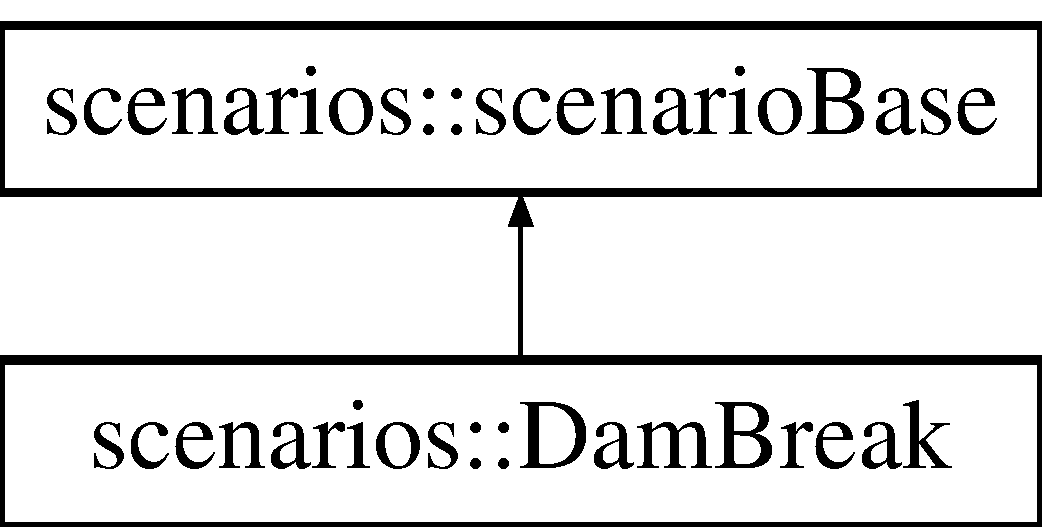
\includegraphics[height=2.000000cm]{classscenarios_1_1DamBreak}
\end{center}
\end{figure}
\subsection*{Public Member Functions}
\begin{DoxyCompactItemize}
\item 
\hyperlink{classscenarios_1_1DamBreak_a7bbd8931d94ea4f001061bde5cb0c57b}{Dam\-Break} (unsigned int size)
\item 
unsigned int \hyperlink{classscenarios_1_1DamBreak_a16c6bc54260b58f539677c4500130223}{get\-Height} (unsigned int pos)
\item 
T \hyperlink{classscenarios_1_1DamBreak_a15d0ac494904dfb9059f0b8685e49e0f}{get\-Momentum} (unsigned int pos)
\item 
T \hyperlink{classscenarios_1_1DamBreak_a4ca1a408aa07a2c3ac0a5613f9d06b7d}{get\-Cell\-Size} ()
\end{DoxyCompactItemize}
\subsection*{Additional Inherited Members}


\subsection{Constructor \& Destructor Documentation}
\hypertarget{classscenarios_1_1DamBreak_a7bbd8931d94ea4f001061bde5cb0c57b}{\index{scenarios\-::\-Dam\-Break@{scenarios\-::\-Dam\-Break}!Dam\-Break@{Dam\-Break}}
\index{Dam\-Break@{Dam\-Break}!scenarios::DamBreak@{scenarios\-::\-Dam\-Break}}
\subsubsection[{Dam\-Break}]{\setlength{\rightskip}{0pt plus 5cm}scenarios\-::\-Dam\-Break\-::\-Dam\-Break (
\begin{DoxyParamCaption}
\item[{unsigned int}]{size}
\end{DoxyParamCaption}
)\hspace{0.3cm}{\ttfamily [inline]}}}\label{classscenarios_1_1DamBreak_a7bbd8931d94ea4f001061bde5cb0c57b}
Constructor for the scenario


\begin{DoxyParams}{Parameters}
{\em size} & The amount of cells which are simulated \\
\hline
\end{DoxyParams}


\subsection{Member Function Documentation}
\hypertarget{classscenarios_1_1DamBreak_a4ca1a408aa07a2c3ac0a5613f9d06b7d}{\index{scenarios\-::\-Dam\-Break@{scenarios\-::\-Dam\-Break}!get\-Cell\-Size@{get\-Cell\-Size}}
\index{get\-Cell\-Size@{get\-Cell\-Size}!scenarios::DamBreak@{scenarios\-::\-Dam\-Break}}
\subsubsection[{get\-Cell\-Size}]{\setlength{\rightskip}{0pt plus 5cm}T scenarios\-::\-Dam\-Break\-::get\-Cell\-Size (
\begin{DoxyParamCaption}
{}
\end{DoxyParamCaption}
)\hspace{0.3cm}{\ttfamily [inline]}, {\ttfamily [virtual]}}}\label{classscenarios_1_1DamBreak_a4ca1a408aa07a2c3ac0a5613f9d06b7d}
\begin{DoxyReturn}{Returns}
Cell size of one cell (= domain size/number of cells) 
\end{DoxyReturn}


Reimplemented from \hyperlink{classscenarios_1_1scenarioBase_a76f3d6f7004dda1344e62bb095d7daca}{scenarios\-::scenario\-Base}.

\hypertarget{classscenarios_1_1DamBreak_a16c6bc54260b58f539677c4500130223}{\index{scenarios\-::\-Dam\-Break@{scenarios\-::\-Dam\-Break}!get\-Height@{get\-Height}}
\index{get\-Height@{get\-Height}!scenarios::DamBreak@{scenarios\-::\-Dam\-Break}}
\subsubsection[{get\-Height}]{\setlength{\rightskip}{0pt plus 5cm}unsigned int scenarios\-::\-Dam\-Break\-::get\-Height (
\begin{DoxyParamCaption}
\item[{unsigned int}]{pos}
\end{DoxyParamCaption}
)\hspace{0.3cm}{\ttfamily [inline]}, {\ttfamily [virtual]}}}\label{classscenarios_1_1DamBreak_a16c6bc54260b58f539677c4500130223}
\begin{DoxyReturn}{Returns}
Initial water height at pos 
\end{DoxyReturn}


Reimplemented from \hyperlink{classscenarios_1_1scenarioBase_ab4b832324300d6921467af8f71b646c2}{scenarios\-::scenario\-Base}.

\hypertarget{classscenarios_1_1DamBreak_a15d0ac494904dfb9059f0b8685e49e0f}{\index{scenarios\-::\-Dam\-Break@{scenarios\-::\-Dam\-Break}!get\-Momentum@{get\-Momentum}}
\index{get\-Momentum@{get\-Momentum}!scenarios::DamBreak@{scenarios\-::\-Dam\-Break}}
\subsubsection[{get\-Momentum}]{\setlength{\rightskip}{0pt plus 5cm}T scenarios\-::\-Dam\-Break\-::get\-Momentum (
\begin{DoxyParamCaption}
\item[{unsigned int}]{pos}
\end{DoxyParamCaption}
)\hspace{0.3cm}{\ttfamily [inline]}, {\ttfamily [virtual]}}}\label{classscenarios_1_1DamBreak_a15d0ac494904dfb9059f0b8685e49e0f}
Returns the initial momentum at a given cell


\begin{DoxyParams}{Parameters}
{\em pos} & The index of the cell\\
\hline
\end{DoxyParams}
\begin{DoxyReturn}{Returns}
The momentum at the specified cell 
\end{DoxyReturn}


Reimplemented from \hyperlink{classscenarios_1_1scenarioBase_a21147d04c54908772ea2d060de49327f}{scenarios\-::scenario\-Base}.



The documentation for this class was generated from the following file\-:\begin{DoxyCompactItemize}
\item 
src/scenarios/\hyperlink{dambreak_8h}{dambreak.\-h}\end{DoxyCompactItemize}

\hypertarget{classsolver_1_1FWave}{\section{solver\-:\-:F\-Wave$<$ T $>$ Class Template Reference}
\label{classsolver_1_1FWave}\index{solver\-::\-F\-Wave$<$ T $>$@{solver\-::\-F\-Wave$<$ T $>$}}
}


{\ttfamily \#include $<$F\-Wave.\-hpp$>$}

\subsection*{Public Member Functions}
\begin{DoxyCompactItemize}
\item 
\hyperlink{classsolver_1_1FWave_a446e2721d799afa5612a3a2b8c30d668}{F\-Wave} ()
\item 
void \hyperlink{classsolver_1_1FWave_afb800cb94c48af043ac828c9d730ae63}{compute\-Net\-Updates} (T i\-\_\-h\-\_\-l, T i\-\_\-h\-\_\-r, T i\-\_\-hu\-\_\-l, T i\-\_\-hu\-\_\-r, T i\-\_\-b\-\_\-l, T i\-\_\-b\-\_\-r, T \&o\-\_\-h\-\_\-l, T \&o\-\_\-h\-\_\-r, T \&o\-\_\-hu\-\_\-l, T \&o\-\_\-hu\-\_\-r, T \&o\-\_\-max\-\_\-ws)
\end{DoxyCompactItemize}


\subsection{Detailed Description}
\subsubsection*{template$<$typename T$>$class solver\-::\-F\-Wave$<$ T $>$}

Simple solver used to compute net udates for a given set of height, momentum and bathymetry values 

\subsection{Constructor \& Destructor Documentation}
\hypertarget{classsolver_1_1FWave_a446e2721d799afa5612a3a2b8c30d668}{\index{solver\-::\-F\-Wave@{solver\-::\-F\-Wave}!F\-Wave@{F\-Wave}}
\index{F\-Wave@{F\-Wave}!solver::FWave@{solver\-::\-F\-Wave}}
\subsubsection[{F\-Wave}]{\setlength{\rightskip}{0pt plus 5cm}template$<$typename T$>$ {\bf solver\-::\-F\-Wave}$<$ T $>$\-::{\bf F\-Wave} (
\begin{DoxyParamCaption}
{}
\end{DoxyParamCaption}
)\hspace{0.3cm}{\ttfamily [inline]}}}\label{classsolver_1_1FWave_a446e2721d799afa5612a3a2b8c30d668}
The default constructor just setting gravity 

\subsection{Member Function Documentation}
\hypertarget{classsolver_1_1FWave_afb800cb94c48af043ac828c9d730ae63}{\index{solver\-::\-F\-Wave@{solver\-::\-F\-Wave}!compute\-Net\-Updates@{compute\-Net\-Updates}}
\index{compute\-Net\-Updates@{compute\-Net\-Updates}!solver::FWave@{solver\-::\-F\-Wave}}
\subsubsection[{compute\-Net\-Updates}]{\setlength{\rightskip}{0pt plus 5cm}template$<$typename T$>$ void {\bf solver\-::\-F\-Wave}$<$ T $>$\-::compute\-Net\-Updates (
\begin{DoxyParamCaption}
\item[{T}]{i\-\_\-h\-\_\-l, }
\item[{T}]{i\-\_\-h\-\_\-r, }
\item[{T}]{i\-\_\-hu\-\_\-l, }
\item[{T}]{i\-\_\-hu\-\_\-r, }
\item[{T}]{i\-\_\-b\-\_\-l, }
\item[{T}]{i\-\_\-b\-\_\-r, }
\item[{T \&}]{o\-\_\-h\-\_\-l, }
\item[{T \&}]{o\-\_\-h\-\_\-r, }
\item[{T \&}]{o\-\_\-hu\-\_\-l, }
\item[{T \&}]{o\-\_\-hu\-\_\-r, }
\item[{T \&}]{o\-\_\-max\-\_\-ws}
\end{DoxyParamCaption}
)\hspace{0.3cm}{\ttfamily [inline]}}}\label{classsolver_1_1FWave_afb800cb94c48af043ac828c9d730ae63}
Computes the next timesteps net updates


\begin{DoxyParams}{Parameters}
{\em i\-\_\-h\-\_\-l} & the height on the left cell of the edge \\
\hline
{\em i\-\_\-h\-\_\-r} & the height on the right cell of the edge \\
\hline
{\em i\-\_\-hu\-\_\-l} & the momentum on the left cell of the edge \\
\hline
{\em i\-\_\-hu\-\_\-r} & the momentum on the right cell of the edge \\
\hline
{\em i\-\_\-b\-\_\-l} & the bathymetry on the left cell of the edge \\
\hline
{\em i\-\_\-b\-\_\-r} & the bathymetry on the right cell of the edge\\
\hline
{\em o\-\_\-h\-\_\-l} & output\-: the height update for the left cell \\
\hline
{\em o\-\_\-h\-\_\-r} & output\-: the height update for the right cell \\
\hline
{\em o\-\_\-hu\-\_\-l} & output\-: the momentum update for the left cell \\
\hline
{\em o\-\_\-hu\-\_\-r} & output\-: the momentum update for the right cell \\
\hline
{\em o\-\_\-max\-\_\-wd} & output\-: the maximum wavespeed (which is the maximum of the left and right wave speed) \\
\hline
\end{DoxyParams}


The documentation for this class was generated from the following file\-:\begin{DoxyCompactItemize}
\item 
submodules/solver/F\-Wave.\-hpp\end{DoxyCompactItemize}

\hypertarget{classFWaveTest}{\section{F\-Wave\-Test Class Reference}
\label{classFWaveTest}\index{F\-Wave\-Test@{F\-Wave\-Test}}
}
Inheritance diagram for F\-Wave\-Test\-:\begin{figure}[H]
\begin{center}
\leavevmode
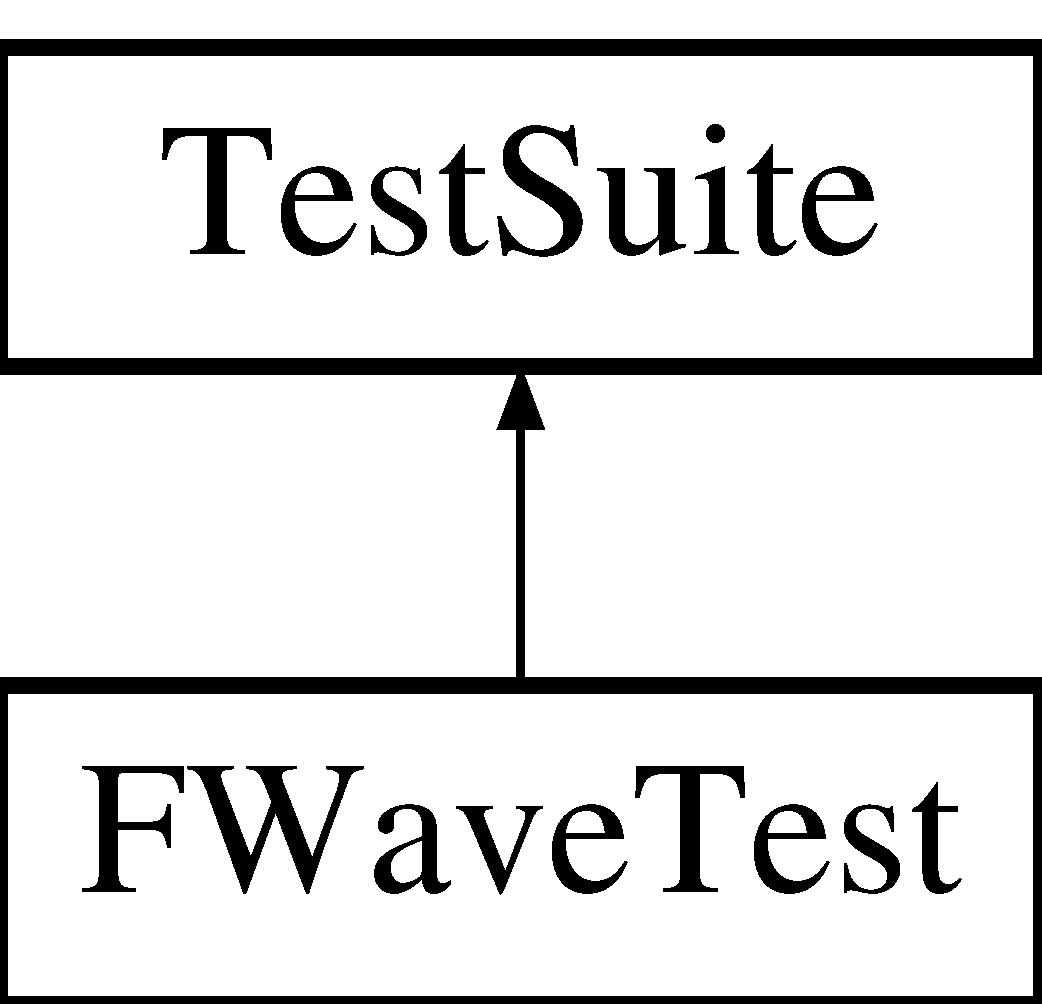
\includegraphics[height=2.000000cm]{classFWaveTest}
\end{center}
\end{figure}
\subsection*{Public Member Functions}
\begin{DoxyCompactItemize}
\item 
void \hyperlink{classFWaveTest_aadefc508d0a1d5e07f9c42bcf5ac7315}{test\-\_\-steady\-\_\-states} (void)
\item 
void \hyperlink{classFWaveTest_a1485f6c0377d6b94da24586b9a39e600}{test\-\_\-both\-\_\-lamda\-\_\-pos\-\_\-neg} (void)
\end{DoxyCompactItemize}


\subsection{Member Function Documentation}
\hypertarget{classFWaveTest_a1485f6c0377d6b94da24586b9a39e600}{\index{F\-Wave\-Test@{F\-Wave\-Test}!test\-\_\-both\-\_\-lamda\-\_\-pos\-\_\-neg@{test\-\_\-both\-\_\-lamda\-\_\-pos\-\_\-neg}}
\index{test\-\_\-both\-\_\-lamda\-\_\-pos\-\_\-neg@{test\-\_\-both\-\_\-lamda\-\_\-pos\-\_\-neg}!FWaveTest@{F\-Wave\-Test}}
\subsubsection[{test\-\_\-both\-\_\-lamda\-\_\-pos\-\_\-neg}]{\setlength{\rightskip}{0pt plus 5cm}void F\-Wave\-Test\-::test\-\_\-both\-\_\-lamda\-\_\-pos\-\_\-neg (
\begin{DoxyParamCaption}
\item[{void}]{}
\end{DoxyParamCaption}
)\hspace{0.3cm}{\ttfamily [inline]}}}\label{classFWaveTest_a1485f6c0377d6b94da24586b9a39e600}
Tests correctness for \mbox{[}Lambda1 $<$ 0 \&\& Lambda 2 $<$ 0\mbox{]} and \mbox{[}Lambda1 $>$ 0 \&\& Lambda 2 $>$ 0\mbox{]} \hypertarget{classFWaveTest_aadefc508d0a1d5e07f9c42bcf5ac7315}{\index{F\-Wave\-Test@{F\-Wave\-Test}!test\-\_\-steady\-\_\-states@{test\-\_\-steady\-\_\-states}}
\index{test\-\_\-steady\-\_\-states@{test\-\_\-steady\-\_\-states}!FWaveTest@{F\-Wave\-Test}}
\subsubsection[{test\-\_\-steady\-\_\-states}]{\setlength{\rightskip}{0pt plus 5cm}void F\-Wave\-Test\-::test\-\_\-steady\-\_\-states (
\begin{DoxyParamCaption}
\item[{void}]{}
\end{DoxyParamCaption}
)\hspace{0.3cm}{\ttfamily [inline]}}}\label{classFWaveTest_aadefc508d0a1d5e07f9c42bcf5ac7315}
Tests 10000 steady states 

The documentation for this class was generated from the following file\-:\begin{DoxyCompactItemize}
\item 
Cxx\-Tests/F\-Wave\-\_\-testsuite.\-t.\-h\end{DoxyCompactItemize}

\hypertarget{classtools_1_1Logger}{\section{tools\-:\-:Logger Class Reference}
\label{classtools_1_1Logger}\index{tools\-::\-Logger@{tools\-::\-Logger}}
}
\subsection*{Public Types}
\begin{DoxyCompactItemize}
\item 
enum {\bfseries Level} \{ {\bfseries I\-N\-F\-O}, 
{\bfseries W\-A\-R\-N\-I\-N\-G}, 
{\bfseries E\-R\-R\-O\-R}
 \}
\end{DoxyCompactItemize}
\subsection*{Public Member Functions}
\begin{DoxyCompactItemize}
\item 
\hypertarget{classtools_1_1Logger_a636053141af12bcbfb816113081c62bc}{void {\bfseries set\-Output\-Stream} (std\-::ostream \&output)}\label{classtools_1_1Logger_a636053141af12bcbfb816113081c62bc}

\item 
\hypertarget{classtools_1_1Logger_a03851adbc4399c2c0c0e0f85fc6a6ef0}{void {\bfseries log} (std\-::string \&message, Level level=I\-N\-F\-O)}\label{classtools_1_1Logger_a03851adbc4399c2c0c0e0f85fc6a6ef0}

\item 
\hypertarget{classtools_1_1Logger_a3fdf70d6ab949dd8483ed5bcd49ce420}{void {\bfseries log} (const char $\ast$message, Level level=I\-N\-F\-O)}\label{classtools_1_1Logger_a3fdf70d6ab949dd8483ed5bcd49ce420}

\item 
\hypertarget{classtools_1_1Logger_ac389acff12d26dbd3fc625c547ac04c7}{void {\bfseries info} (std\-::string \&message)}\label{classtools_1_1Logger_ac389acff12d26dbd3fc625c547ac04c7}

\item 
\hypertarget{classtools_1_1Logger_a24a476db1d106f5d4b13a9fa39d1b0dc}{void {\bfseries info} (const char $\ast$message)}\label{classtools_1_1Logger_a24a476db1d106f5d4b13a9fa39d1b0dc}

\item 
\hypertarget{classtools_1_1Logger_a91efb6571b01077f2dfb55c47aaf253e}{std\-::ostream \& {\bfseries info} ()}\label{classtools_1_1Logger_a91efb6571b01077f2dfb55c47aaf253e}

\item 
\hypertarget{classtools_1_1Logger_a5d3ae06c39df8abc23c2d81de79c882f}{void {\bfseries warning} (std\-::string \&message)}\label{classtools_1_1Logger_a5d3ae06c39df8abc23c2d81de79c882f}

\item 
\hypertarget{classtools_1_1Logger_abc773c41c59d9afbb620476341f95718}{void {\bfseries warning} (const char $\ast$message)}\label{classtools_1_1Logger_abc773c41c59d9afbb620476341f95718}

\item 
\hypertarget{classtools_1_1Logger_a8aafc0559791caa80a1f655d4da3e411}{std\-::ostream \& {\bfseries warning} ()}\label{classtools_1_1Logger_a8aafc0559791caa80a1f655d4da3e411}

\item 
\hypertarget{classtools_1_1Logger_ae7a4f4f4ad7ebf58e89e46f59c124dac}{void {\bfseries error} (std\-::string \&message)}\label{classtools_1_1Logger_ae7a4f4f4ad7ebf58e89e46f59c124dac}

\item 
\hypertarget{classtools_1_1Logger_a769bbaa6d8dcc4a10803107c01d1a42c}{void {\bfseries error} (const char $\ast$message)}\label{classtools_1_1Logger_a769bbaa6d8dcc4a10803107c01d1a42c}

\item 
{\footnotesize template$<$typename T $>$ }\\\hyperlink{classtools_1_1Logger}{Logger} \& \hyperlink{classtools_1_1Logger_a329a9574f28452d55118911d2ce428f8}{operator$<$$<$} (T value)
\item 
\hyperlink{classtools_1_1Logger}{Logger} \& \hyperlink{classtools_1_1Logger_aad70622a440e19c348291a46be9d0751}{operator$<$$<$} (std\-::ostream \&($\ast$func)(std\-::ostream \&))
\end{DoxyCompactItemize}
\subsection*{Static Public Attributes}
\begin{DoxyCompactItemize}
\item 
\hypertarget{classtools_1_1Logger_a341eaab3865b60362db6736c2e2b7c68}{static \hyperlink{classtools_1_1Logger}{Logger} {\bfseries logger}}\label{classtools_1_1Logger_a341eaab3865b60362db6736c2e2b7c68}

\end{DoxyCompactItemize}


\subsection{Member Function Documentation}
\hypertarget{classtools_1_1Logger_a329a9574f28452d55118911d2ce428f8}{\index{tools\-::\-Logger@{tools\-::\-Logger}!operator$<$$<$@{operator$<$$<$}}
\index{operator$<$$<$@{operator$<$$<$}!tools::Logger@{tools\-::\-Logger}}
\subsubsection[{operator$<$$<$}]{\setlength{\rightskip}{0pt plus 5cm}template$<$typename T $>$ {\bf Logger}\& tools\-::\-Logger\-::operator$<$$<$ (
\begin{DoxyParamCaption}
\item[{T}]{value}
\end{DoxyParamCaption}
)\hspace{0.3cm}{\ttfamily [inline]}}}\label{classtools_1_1Logger_a329a9574f28452d55118911d2ce428f8}
Can be used to print arbitrary info messages. Does not append std\-::endl. \hypertarget{classtools_1_1Logger_aad70622a440e19c348291a46be9d0751}{\index{tools\-::\-Logger@{tools\-::\-Logger}!operator$<$$<$@{operator$<$$<$}}
\index{operator$<$$<$@{operator$<$$<$}!tools::Logger@{tools\-::\-Logger}}
\subsubsection[{operator$<$$<$}]{\setlength{\rightskip}{0pt plus 5cm}{\bf Logger}\& tools\-::\-Logger\-::operator$<$$<$ (
\begin{DoxyParamCaption}
\item[{std\-::ostream \&($\ast$)(std\-::ostream \&)}]{func}
\end{DoxyParamCaption}
)\hspace{0.3cm}{\ttfamily [inline]}}}\label{classtools_1_1Logger_aad70622a440e19c348291a46be9d0751}
Allow to print std\-::endl 

The documentation for this class was generated from the following files\-:\begin{DoxyCompactItemize}
\item 
src/tools/\hyperlink{logger_8h}{logger.\-h}\item 
src/tools/\hyperlink{logger_8cpp}{logger.\-cpp}\end{DoxyCompactItemize}

\hypertarget{classscenarios_1_1Rare}{\section{scenarios\-:\-:Rare Class Reference}
\label{classscenarios_1_1Rare}\index{scenarios\-::\-Rare@{scenarios\-::\-Rare}}
}
Inheritance diagram for scenarios\-:\-:Rare\-:\begin{figure}[H]
\begin{center}
\leavevmode
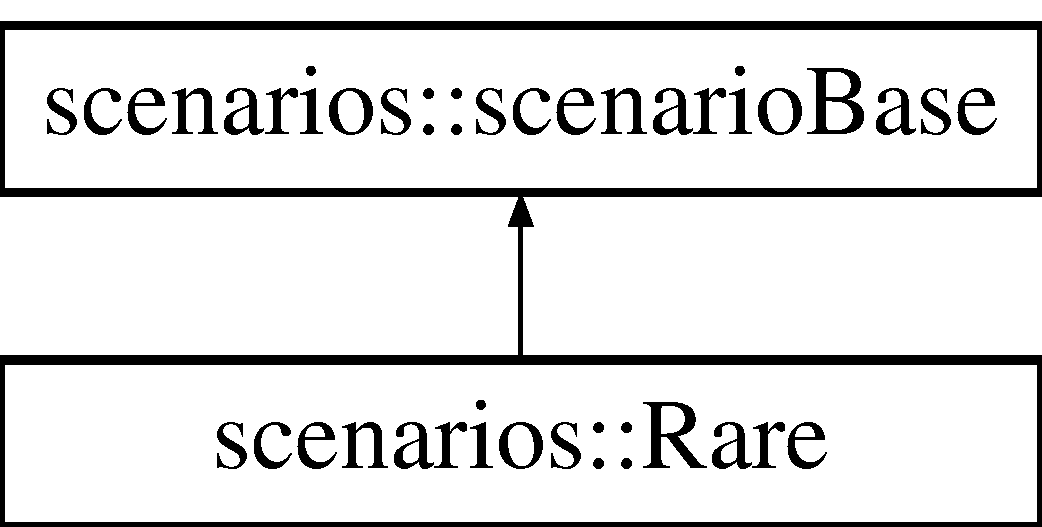
\includegraphics[height=2.000000cm]{classscenarios_1_1Rare}
\end{center}
\end{figure}
\subsection*{Public Member Functions}
\begin{DoxyCompactItemize}
\item 
\hyperlink{classscenarios_1_1Rare_af503e3e602a16fe2fa3bcdbe5ea4b61e}{Rare} (unsigned int size)
\item 
T \hyperlink{classscenarios_1_1Rare_adac016d86c243d8a08227927cabc368c}{get\-Height} (unsigned int pos)
\item 
T \hyperlink{classscenarios_1_1Rare_a33b6c2b5a5d81d7e1a1f5b0c0028ac2d}{get\-Momentum} (unsigned int pos)
\end{DoxyCompactItemize}
\subsection*{Additional Inherited Members}


\subsection{Constructor \& Destructor Documentation}
\hypertarget{classscenarios_1_1Rare_af503e3e602a16fe2fa3bcdbe5ea4b61e}{\index{scenarios\-::\-Rare@{scenarios\-::\-Rare}!Rare@{Rare}}
\index{Rare@{Rare}!scenarios::Rare@{scenarios\-::\-Rare}}
\subsubsection[{Rare}]{\setlength{\rightskip}{0pt plus 5cm}scenarios\-::\-Rare\-::\-Rare (
\begin{DoxyParamCaption}
\item[{unsigned int}]{size}
\end{DoxyParamCaption}
)\hspace{0.3cm}{\ttfamily [inline]}}}\label{classscenarios_1_1Rare_af503e3e602a16fe2fa3bcdbe5ea4b61e}
Constructor for the scenario


\begin{DoxyParams}{Parameters}
{\em size} & The amount of cells which are simulated \\
\hline
\end{DoxyParams}


\subsection{Member Function Documentation}
\hypertarget{classscenarios_1_1Rare_adac016d86c243d8a08227927cabc368c}{\index{scenarios\-::\-Rare@{scenarios\-::\-Rare}!get\-Height@{get\-Height}}
\index{get\-Height@{get\-Height}!scenarios::Rare@{scenarios\-::\-Rare}}
\subsubsection[{get\-Height}]{\setlength{\rightskip}{0pt plus 5cm}T scenarios\-::\-Rare\-::get\-Height (
\begin{DoxyParamCaption}
\item[{unsigned int}]{pos}
\end{DoxyParamCaption}
)\hspace{0.3cm}{\ttfamily [inline]}, {\ttfamily [virtual]}}}\label{classscenarios_1_1Rare_adac016d86c243d8a08227927cabc368c}
Returns the initial height at a given cell


\begin{DoxyParams}{Parameters}
{\em pos} & The index of the cell\\
\hline
\end{DoxyParams}
\begin{DoxyReturn}{Returns}
The height of the specified cell 
\end{DoxyReturn}


Reimplemented from \hyperlink{classscenarios_1_1scenarioBase_abf012aedec3ba04bbb5f84142ba568ca}{scenarios\-::scenario\-Base}.

\hypertarget{classscenarios_1_1Rare_a33b6c2b5a5d81d7e1a1f5b0c0028ac2d}{\index{scenarios\-::\-Rare@{scenarios\-::\-Rare}!get\-Momentum@{get\-Momentum}}
\index{get\-Momentum@{get\-Momentum}!scenarios::Rare@{scenarios\-::\-Rare}}
\subsubsection[{get\-Momentum}]{\setlength{\rightskip}{0pt plus 5cm}T scenarios\-::\-Rare\-::get\-Momentum (
\begin{DoxyParamCaption}
\item[{unsigned int}]{pos}
\end{DoxyParamCaption}
)\hspace{0.3cm}{\ttfamily [inline]}, {\ttfamily [virtual]}}}\label{classscenarios_1_1Rare_a33b6c2b5a5d81d7e1a1f5b0c0028ac2d}
Returns the initial momentum at a given cell


\begin{DoxyParams}{Parameters}
{\em pos} & The index of the cell\\
\hline
\end{DoxyParams}
\begin{DoxyReturn}{Returns}
The momentum at the specified cell 
\end{DoxyReturn}


Reimplemented from \hyperlink{classscenarios_1_1scenarioBase_a21147d04c54908772ea2d060de49327f}{scenarios\-::scenario\-Base}.



The documentation for this class was generated from the following file\-:\begin{DoxyCompactItemize}
\item 
src/scenarios/rare.\-h\end{DoxyCompactItemize}

\hypertarget{classscenarios_1_1scenarioBase}{\section{scenarios\-:\-:scenario\-Base Class Reference}
\label{classscenarios_1_1scenarioBase}\index{scenarios\-::scenario\-Base@{scenarios\-::scenario\-Base}}
}
Inheritance diagram for scenarios\-:\-:scenario\-Base\-:\begin{figure}[H]
\begin{center}
\leavevmode
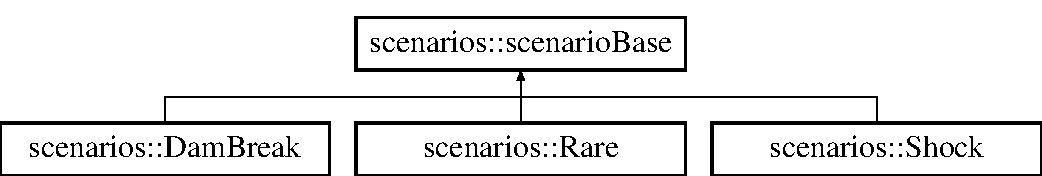
\includegraphics[height=2.000000cm]{classscenarios_1_1scenarioBase}
\end{center}
\end{figure}
\subsection*{Public Member Functions}
\begin{DoxyCompactItemize}
\item 
\hyperlink{classscenarios_1_1scenarioBase_adb8ed429de97c9d478460906e9d66801}{scenario\-Base} (unsigned int size)
\item 
virtual T \hyperlink{classscenarios_1_1scenarioBase_abf012aedec3ba04bbb5f84142ba568ca}{get\-Height} (unsigned int pos)
\item 
virtual T \hyperlink{classscenarios_1_1scenarioBase_a21147d04c54908772ea2d060de49327f}{get\-Momentum} (unsigned int pos)
\item 
virtual T \hyperlink{classscenarios_1_1scenarioBase_a76f3d6f7004dda1344e62bb095d7daca}{get\-Cell\-Size} ()
\end{DoxyCompactItemize}
\subsection*{Protected Attributes}
\begin{DoxyCompactItemize}
\item 
const unsigned int \hyperlink{classscenarios_1_1scenarioBase_a67c277c3749ab83d0cb1749200a38791}{m\-\_\-size}
\end{DoxyCompactItemize}


\subsection{Constructor \& Destructor Documentation}
\hypertarget{classscenarios_1_1scenarioBase_adb8ed429de97c9d478460906e9d66801}{\index{scenarios\-::scenario\-Base@{scenarios\-::scenario\-Base}!scenario\-Base@{scenario\-Base}}
\index{scenario\-Base@{scenario\-Base}!scenarios::scenarioBase@{scenarios\-::scenario\-Base}}
\subsubsection[{scenario\-Base}]{\setlength{\rightskip}{0pt plus 5cm}scenarios\-::scenario\-Base\-::scenario\-Base (
\begin{DoxyParamCaption}
\item[{unsigned int}]{size}
\end{DoxyParamCaption}
)\hspace{0.3cm}{\ttfamily [inline]}}}\label{classscenarios_1_1scenarioBase_adb8ed429de97c9d478460906e9d66801}
Constructor for the scenario


\begin{DoxyParams}{Parameters}
{\em size} & The amount of cells which are simulated \\
\hline
\end{DoxyParams}


\subsection{Member Function Documentation}
\hypertarget{classscenarios_1_1scenarioBase_a76f3d6f7004dda1344e62bb095d7daca}{\index{scenarios\-::scenario\-Base@{scenarios\-::scenario\-Base}!get\-Cell\-Size@{get\-Cell\-Size}}
\index{get\-Cell\-Size@{get\-Cell\-Size}!scenarios::scenarioBase@{scenarios\-::scenario\-Base}}
\subsubsection[{get\-Cell\-Size}]{\setlength{\rightskip}{0pt plus 5cm}virtual T scenarios\-::scenario\-Base\-::get\-Cell\-Size (
\begin{DoxyParamCaption}
{}
\end{DoxyParamCaption}
)\hspace{0.3cm}{\ttfamily [inline]}, {\ttfamily [virtual]}}}\label{classscenarios_1_1scenarioBase_a76f3d6f7004dda1344e62bb095d7daca}
Returns the width of each cell

\begin{DoxyReturn}{Returns}
Width of one cell 
\end{DoxyReturn}


Reimplemented in \hyperlink{classscenarios_1_1DamBreak_a4ca1a408aa07a2c3ac0a5613f9d06b7d}{scenarios\-::\-Dam\-Break}.

\hypertarget{classscenarios_1_1scenarioBase_abf012aedec3ba04bbb5f84142ba568ca}{\index{scenarios\-::scenario\-Base@{scenarios\-::scenario\-Base}!get\-Height@{get\-Height}}
\index{get\-Height@{get\-Height}!scenarios::scenarioBase@{scenarios\-::scenario\-Base}}
\subsubsection[{get\-Height}]{\setlength{\rightskip}{0pt plus 5cm}virtual T scenarios\-::scenario\-Base\-::get\-Height (
\begin{DoxyParamCaption}
\item[{unsigned int}]{pos}
\end{DoxyParamCaption}
)\hspace{0.3cm}{\ttfamily [inline]}, {\ttfamily [virtual]}}}\label{classscenarios_1_1scenarioBase_abf012aedec3ba04bbb5f84142ba568ca}
Returns the initial height at a given cell


\begin{DoxyParams}{Parameters}
{\em pos} & The index of the cell\\
\hline
\end{DoxyParams}
\begin{DoxyReturn}{Returns}
The height of the specified cell 
\end{DoxyReturn}


Reimplemented in \hyperlink{classscenarios_1_1DamBreak_adb2898029dbd63464bbbb9367b58b075}{scenarios\-::\-Dam\-Break}, \hyperlink{classscenarios_1_1Shock_af907fcea7801db13c3f4b281c5b1326a}{scenarios\-::\-Shock}, and \hyperlink{classscenarios_1_1Rare_adac016d86c243d8a08227927cabc368c}{scenarios\-::\-Rare}.

\hypertarget{classscenarios_1_1scenarioBase_a21147d04c54908772ea2d060de49327f}{\index{scenarios\-::scenario\-Base@{scenarios\-::scenario\-Base}!get\-Momentum@{get\-Momentum}}
\index{get\-Momentum@{get\-Momentum}!scenarios::scenarioBase@{scenarios\-::scenario\-Base}}
\subsubsection[{get\-Momentum}]{\setlength{\rightskip}{0pt plus 5cm}virtual T scenarios\-::scenario\-Base\-::get\-Momentum (
\begin{DoxyParamCaption}
\item[{unsigned int}]{pos}
\end{DoxyParamCaption}
)\hspace{0.3cm}{\ttfamily [inline]}, {\ttfamily [virtual]}}}\label{classscenarios_1_1scenarioBase_a21147d04c54908772ea2d060de49327f}
Returns the initial momentum at a given cell


\begin{DoxyParams}{Parameters}
{\em pos} & The index of the cell\\
\hline
\end{DoxyParams}
\begin{DoxyReturn}{Returns}
The momentum at the specified cell 
\end{DoxyReturn}


Reimplemented in \hyperlink{classscenarios_1_1DamBreak_a15d0ac494904dfb9059f0b8685e49e0f}{scenarios\-::\-Dam\-Break}, \hyperlink{classscenarios_1_1Shock_a89b88a5223ae0f82178ac63c724a6d91}{scenarios\-::\-Shock}, and \hyperlink{classscenarios_1_1Rare_a33b6c2b5a5d81d7e1a1f5b0c0028ac2d}{scenarios\-::\-Rare}.



\subsection{Member Data Documentation}
\hypertarget{classscenarios_1_1scenarioBase_a67c277c3749ab83d0cb1749200a38791}{\index{scenarios\-::scenario\-Base@{scenarios\-::scenario\-Base}!m\-\_\-size@{m\-\_\-size}}
\index{m\-\_\-size@{m\-\_\-size}!scenarios::scenarioBase@{scenarios\-::scenario\-Base}}
\subsubsection[{m\-\_\-size}]{\setlength{\rightskip}{0pt plus 5cm}const unsigned int scenarios\-::scenario\-Base\-::m\-\_\-size\hspace{0.3cm}{\ttfamily [protected]}}}\label{classscenarios_1_1scenarioBase_a67c277c3749ab83d0cb1749200a38791}
Number of cells 

The documentation for this class was generated from the following file\-:\begin{DoxyCompactItemize}
\item 
src/scenarios/scenario.\-h\end{DoxyCompactItemize}

\hypertarget{classscenarios_1_1Shock}{\section{scenarios\-:\-:Shock Class Reference}
\label{classscenarios_1_1Shock}\index{scenarios\-::\-Shock@{scenarios\-::\-Shock}}
}


{\ttfamily \#include $<$schock.\-h$>$}

Inheritance diagram for scenarios\-:\-:Shock\-:\begin{figure}[H]
\begin{center}
\leavevmode
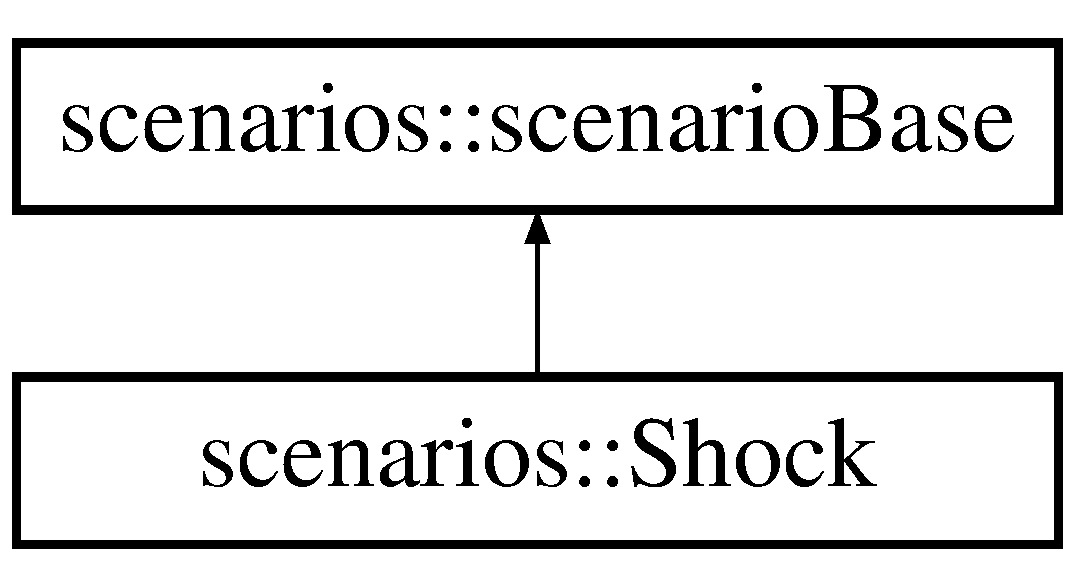
\includegraphics[height=2.000000cm]{classscenarios_1_1Shock}
\end{center}
\end{figure}
\subsection*{Public Member Functions}
\begin{DoxyCompactItemize}
\item 
\hyperlink{classscenarios_1_1Shock_a6c3694a5cfe8968eda7d7f9862e3b035}{Shock} (unsigned int size)
\item 
unsigned int \hyperlink{classscenarios_1_1Shock_a6041f87441e9e04e6f7a9c2fdab12edb}{get\-Height} (unsigned int pos)
\item 
T \hyperlink{classscenarios_1_1Shock_a89b88a5223ae0f82178ac63c724a6d91}{get\-Momentum} (unsigned int pos)
\end{DoxyCompactItemize}
\subsection*{Additional Inherited Members}


\subsection{Detailed Description}
This class offers the setup for a shock-\/shock scenario. The water walls are located at the outer sides (facing inwards) with a distance of one quarter of the whole amount of cells to the edges 

\subsection{Constructor \& Destructor Documentation}
\hypertarget{classscenarios_1_1Shock_a6c3694a5cfe8968eda7d7f9862e3b035}{\index{scenarios\-::\-Shock@{scenarios\-::\-Shock}!Shock@{Shock}}
\index{Shock@{Shock}!scenarios::Shock@{scenarios\-::\-Shock}}
\subsubsection[{Shock}]{\setlength{\rightskip}{0pt plus 5cm}scenarios\-::\-Shock\-::\-Shock (
\begin{DoxyParamCaption}
\item[{unsigned int}]{size}
\end{DoxyParamCaption}
)\hspace{0.3cm}{\ttfamily [inline]}}}\label{classscenarios_1_1Shock_a6c3694a5cfe8968eda7d7f9862e3b035}
Constructor for the scenario


\begin{DoxyParams}{Parameters}
{\em size} & The amount of cells which are simulated \\
\hline
\end{DoxyParams}


\subsection{Member Function Documentation}
\hypertarget{classscenarios_1_1Shock_a6041f87441e9e04e6f7a9c2fdab12edb}{\index{scenarios\-::\-Shock@{scenarios\-::\-Shock}!get\-Height@{get\-Height}}
\index{get\-Height@{get\-Height}!scenarios::Shock@{scenarios\-::\-Shock}}
\subsubsection[{get\-Height}]{\setlength{\rightskip}{0pt plus 5cm}unsigned int scenarios\-::\-Shock\-::get\-Height (
\begin{DoxyParamCaption}
\item[{unsigned int}]{pos}
\end{DoxyParamCaption}
)\hspace{0.3cm}{\ttfamily [inline]}, {\ttfamily [virtual]}}}\label{classscenarios_1_1Shock_a6041f87441e9e04e6f7a9c2fdab12edb}
Returns the initial height at a given cell


\begin{DoxyParams}{Parameters}
{\em pos} & The index of the cell\\
\hline
\end{DoxyParams}
\begin{DoxyReturn}{Returns}
The height of the specified cell 
\end{DoxyReturn}


Reimplemented from \hyperlink{classscenarios_1_1scenarioBase_ab4b832324300d6921467af8f71b646c2}{scenarios\-::scenario\-Base}.

\hypertarget{classscenarios_1_1Shock_a89b88a5223ae0f82178ac63c724a6d91}{\index{scenarios\-::\-Shock@{scenarios\-::\-Shock}!get\-Momentum@{get\-Momentum}}
\index{get\-Momentum@{get\-Momentum}!scenarios::Shock@{scenarios\-::\-Shock}}
\subsubsection[{get\-Momentum}]{\setlength{\rightskip}{0pt plus 5cm}T scenarios\-::\-Shock\-::get\-Momentum (
\begin{DoxyParamCaption}
\item[{unsigned int}]{pos}
\end{DoxyParamCaption}
)\hspace{0.3cm}{\ttfamily [inline]}, {\ttfamily [virtual]}}}\label{classscenarios_1_1Shock_a89b88a5223ae0f82178ac63c724a6d91}
Returns the initial momentum at a given cell


\begin{DoxyParams}{Parameters}
{\em pos} & The index of the cell\\
\hline
\end{DoxyParams}
\begin{DoxyReturn}{Returns}
The momentum at the specified cell 
\end{DoxyReturn}


Reimplemented from \hyperlink{classscenarios_1_1scenarioBase_a21147d04c54908772ea2d060de49327f}{scenarios\-::scenario\-Base}.



The documentation for this class was generated from the following file\-:\begin{DoxyCompactItemize}
\item 
src/scenarios/schock.\-h\end{DoxyCompactItemize}

\hypertarget{classcxxtest_1_1ToolCxxTestWarning}{\section{cxxtest.\-Tool\-Cxx\-Test\-Warning Class Reference}
\label{classcxxtest_1_1ToolCxxTestWarning}\index{cxxtest.\-Tool\-Cxx\-Test\-Warning@{cxxtest.\-Tool\-Cxx\-Test\-Warning}}
}
Inheritance diagram for cxxtest.\-Tool\-Cxx\-Test\-Warning\-:\begin{figure}[H]
\begin{center}
\leavevmode
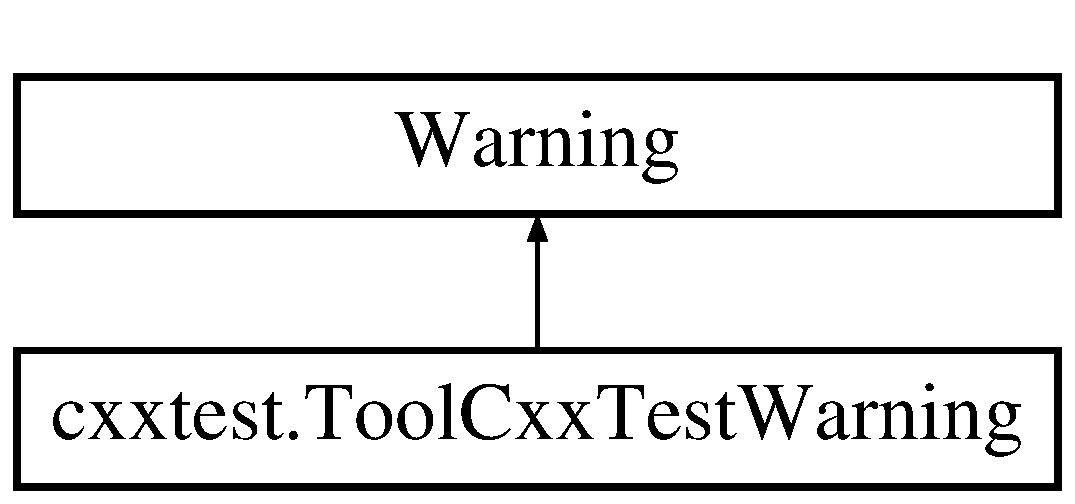
\includegraphics[height=2.000000cm]{classcxxtest_1_1ToolCxxTestWarning}
\end{center}
\end{figure}


The documentation for this class was generated from the following file\-:\begin{DoxyCompactItemize}
\item 
site\-\_\-scons/site\-\_\-tools/cxxtest.\-py\end{DoxyCompactItemize}

\hypertarget{classwriter_1_1VtkWriter}{\section{writer\-:\-:Vtk\-Writer Class Reference}
\label{classwriter_1_1VtkWriter}\index{writer\-::\-Vtk\-Writer@{writer\-::\-Vtk\-Writer}}
}


{\ttfamily \#include $<$Vtk\-Writer.\-h$>$}

\subsection*{Public Member Functions}
\begin{DoxyCompactItemize}
\item 
\hypertarget{classwriter_1_1VtkWriter_a57c97e5e03496b7af25e202e85bbc82c}{{\bfseries Vtk\-Writer} (const std\-::string \&basename=\char`\"{}swe1d\char`\"{}, const T cell\-Size=1)}\label{classwriter_1_1VtkWriter_a57c97e5e03496b7af25e202e85bbc82c}

\item 
void \hyperlink{classwriter_1_1VtkWriter_a49e3f57f4a7b4c677919dea1fbd58f18}{write} (const T time, const T $\ast$h, const T $\ast$hu, unsigned int size)
\end{DoxyCompactItemize}


\subsection{Detailed Description}
A writer class that generates vtk files 

\subsection{Member Function Documentation}
\hypertarget{classwriter_1_1VtkWriter_a49e3f57f4a7b4c677919dea1fbd58f18}{\index{writer\-::\-Vtk\-Writer@{writer\-::\-Vtk\-Writer}!write@{write}}
\index{write@{write}!writer::VtkWriter@{writer\-::\-Vtk\-Writer}}
\subsubsection[{write}]{\setlength{\rightskip}{0pt plus 5cm}void writer\-::\-Vtk\-Writer\-::write (
\begin{DoxyParamCaption}
\item[{const T}]{time, }
\item[{const T $\ast$}]{h, }
\item[{const T $\ast$}]{hu, }
\item[{unsigned int}]{size}
\end{DoxyParamCaption}
)\hspace{0.3cm}{\ttfamily [inline]}}}\label{classwriter_1_1VtkWriter_a49e3f57f4a7b4c677919dea1fbd58f18}
Writes all values to vtk file


\begin{DoxyParams}{Parameters}
{\em size} & Number of cells (without boundary values) \\
\hline
\end{DoxyParams}


The documentation for this class was generated from the following file\-:\begin{DoxyCompactItemize}
\item 
src/writer/\hyperlink{VtkWriter_8h}{Vtk\-Writer.\-h}\end{DoxyCompactItemize}

\hypertarget{classWavePropagation}{\section{Wave\-Propagation Class Reference}
\label{classWavePropagation}\index{Wave\-Propagation@{Wave\-Propagation}}
}


{\ttfamily \#include $<$Wave\-Propagation.\-h$>$}

\subsection*{Public Member Functions}
\begin{DoxyCompactItemize}
\item 
\hyperlink{classWavePropagation_ad24b3385c595d77ed4e989bf19cd587d}{Wave\-Propagation} (T $\ast$h, T $\ast$hu, unsigned int size, T cell\-Size)
\item 
T \hyperlink{classWavePropagation_a7e4ccdb5689e8e05c5e05887386d0a63}{compute\-Numerical\-Fluxes} ()
\item 
void \hyperlink{classWavePropagation_ae7b96a1eb21ae248a37afe4d57d01dd9}{update\-Unknowns} (T dt)
\item 
void \hyperlink{classWavePropagation_abdd5acb41399ec0cea238d41b8df1d6b}{set\-Outflow\-Boundary\-Conditions} ()
\end{DoxyCompactItemize}


\subsection{Detailed Description}
Allocated variables\-: unknowns h,hu are defined on grid indices \mbox{[}0,..,n+1\mbox{]} (done by the caller) -\/$>$ computational domain is \mbox{[}1,..,nx\mbox{]} -\/$>$ plus ghost cell layer

net-\/updates are defined for edges with indices \mbox{[}0,..,n\mbox{]}

A left/right net update with index (i-\/1) is located on the edge between cells with index (i-\/1) and (i)\-: 
\begin{DoxyPre}






  *  (i-1)  *   (i)   *






\begin{DoxyVerb}      *
     ***
    *****
      *
      *
\end{DoxyVerb}

   NetUpdatesLeft(i-1)
            or
   NetUpdatesRight(i-1)
\end{DoxyPre}
 

\subsection{Constructor \& Destructor Documentation}
\hypertarget{classWavePropagation_ad24b3385c595d77ed4e989bf19cd587d}{\index{Wave\-Propagation@{Wave\-Propagation}!Wave\-Propagation@{Wave\-Propagation}}
\index{Wave\-Propagation@{Wave\-Propagation}!WavePropagation@{Wave\-Propagation}}
\subsubsection[{Wave\-Propagation}]{\setlength{\rightskip}{0pt plus 5cm}Wave\-Propagation\-::\-Wave\-Propagation (
\begin{DoxyParamCaption}
\item[{T $\ast$}]{h, }
\item[{T $\ast$}]{hu, }
\item[{unsigned int}]{size, }
\item[{T}]{cell\-Size}
\end{DoxyParamCaption}
)\hspace{0.3cm}{\ttfamily [inline]}}}\label{classWavePropagation_ad24b3385c595d77ed4e989bf19cd587d}

\begin{DoxyParams}{Parameters}
{\em size} & Domain size (= number of cells) without ghost cells \\
\hline
{\em cell\-Size} & Size of one cell \\
\hline
\end{DoxyParams}


\subsection{Member Function Documentation}
\hypertarget{classWavePropagation_a7e4ccdb5689e8e05c5e05887386d0a63}{\index{Wave\-Propagation@{Wave\-Propagation}!compute\-Numerical\-Fluxes@{compute\-Numerical\-Fluxes}}
\index{compute\-Numerical\-Fluxes@{compute\-Numerical\-Fluxes}!WavePropagation@{Wave\-Propagation}}
\subsubsection[{compute\-Numerical\-Fluxes}]{\setlength{\rightskip}{0pt plus 5cm}T Wave\-Propagation\-::compute\-Numerical\-Fluxes (
\begin{DoxyParamCaption}
{}
\end{DoxyParamCaption}
)}}\label{classWavePropagation_a7e4ccdb5689e8e05c5e05887386d0a63}
Computes the net-\/updates from the unknowns

\begin{DoxyReturn}{Returns}
The maximum possible time step 
\end{DoxyReturn}
\hypertarget{classWavePropagation_abdd5acb41399ec0cea238d41b8df1d6b}{\index{Wave\-Propagation@{Wave\-Propagation}!set\-Outflow\-Boundary\-Conditions@{set\-Outflow\-Boundary\-Conditions}}
\index{set\-Outflow\-Boundary\-Conditions@{set\-Outflow\-Boundary\-Conditions}!WavePropagation@{Wave\-Propagation}}
\subsubsection[{set\-Outflow\-Boundary\-Conditions}]{\setlength{\rightskip}{0pt plus 5cm}void Wave\-Propagation\-::set\-Outflow\-Boundary\-Conditions (
\begin{DoxyParamCaption}
{}
\end{DoxyParamCaption}
)}}\label{classWavePropagation_abdd5acb41399ec0cea238d41b8df1d6b}
Updates h and hu according to the outflow condition to both boundaries \hypertarget{classWavePropagation_ae7b96a1eb21ae248a37afe4d57d01dd9}{\index{Wave\-Propagation@{Wave\-Propagation}!update\-Unknowns@{update\-Unknowns}}
\index{update\-Unknowns@{update\-Unknowns}!WavePropagation@{Wave\-Propagation}}
\subsubsection[{update\-Unknowns}]{\setlength{\rightskip}{0pt plus 5cm}void Wave\-Propagation\-::update\-Unknowns (
\begin{DoxyParamCaption}
\item[{T}]{dt}
\end{DoxyParamCaption}
)}}\label{classWavePropagation_ae7b96a1eb21ae248a37afe4d57d01dd9}
Update the unknowns with the already computed net-\/updates


\begin{DoxyParams}{Parameters}
{\em dt} & Time step size \\
\hline
\end{DoxyParams}


The documentation for this class was generated from the following files\-:\begin{DoxyCompactItemize}
\item 
src/\hyperlink{WavePropagation_8h}{Wave\-Propagation.\-h}\item 
src/\hyperlink{WavePropagation_8cpp}{Wave\-Propagation.\-cpp}\end{DoxyCompactItemize}

\chapter{File Documentation}
\hypertarget{main_8cpp}{\section{src/main.cpp File Reference}
\label{main_8cpp}\index{src/main.\-cpp@{src/main.\-cpp}}
}
{\ttfamily \#include \char`\"{}types.\-h\char`\"{}}\\*
{\ttfamily \#include \char`\"{}Wave\-Propagation.\-h\char`\"{}}\\*
{\ttfamily \#include \char`\"{}writer/\-Console\-Writer.\-h\char`\"{}}\\*
{\ttfamily \#include \char`\"{}writer/\-Vtk\-Writer.\-h\char`\"{}}\\*
{\ttfamily \#include \char`\"{}tools/args.\-h\char`\"{}}\\*
{\ttfamily \#include $<$cstring$>$}\\*
\subsection*{Functions}
\begin{DoxyCompactItemize}
\item 
\hypertarget{main_8cpp_a3c04138a5bfe5d72780bb7e82a18e627}{int {\bfseries main} (int argc, char $\ast$$\ast$argv)}\label{main_8cpp_a3c04138a5bfe5d72780bb7e82a18e627}

\end{DoxyCompactItemize}


\subsection{Detailed Description}
This file is part of S\-W\-E1\-D

S\-W\-E1\-D is free software\-: you can redistribute it and/or modify it under the terms of the G\-N\-U General Public License as published by the Free Software Foundation, either version 3 of the License, or (at your option) any later version.

S\-W\-E1\-D is distributed in the hope that it will be useful, but W\-I\-T\-H\-O\-U\-T A\-N\-Y W\-A\-R\-R\-A\-N\-T\-Y; without even the implied warranty of M\-E\-R\-C\-H\-A\-N\-T\-A\-B\-I\-L\-I\-T\-Y or F\-I\-T\-N\-E\-S\-S F\-O\-R A P\-A\-R\-T\-I\-C\-U\-L\-A\-R P\-U\-R\-P\-O\-S\-E. See the G\-N\-U General Public License for more details.

You should have received a copy of the G\-N\-U General Public License along with S\-W\-E1\-D. If not, see \href{http://www.gnu.org/licenses/}{\tt http\-://www.\-gnu.\-org/licenses/}.

Diese Datei ist Teil von S\-W\-E1\-D.

S\-W\-E1\-D ist Freie Software\-: Sie koennen es unter den Bedingungen der G\-N\-U General Public License, wie von der Free Software Foundation, Version 3 der Lizenz oder (nach Ihrer Option) jeder spaeteren veroeffentlichten Version, weiterverbreiten und/oder modifizieren.

S\-W\-E1\-D wird in der Hoffnung, dass es nuetzlich sein wird, aber O\-H\-N\-E J\-E\-D\-E G\-E\-W\-A\-E\-H\-E\-L\-E\-I\-S\-T\-U\-N\-G, bereitgestellt; sogar ohne die implizite Gewaehrleistung der M\-A\-R\-K\-T\-F\-A\-E\-H\-I\-G\-K\-E\-I\-T oder E\-I\-G\-N\-U\-N\-G F\-U\-E\-R E\-I\-N\-E\-N B\-E\-S\-T\-I\-M\-M\-T\-E\-N Z\-W\-E\-C\-K. Siehe die G\-N\-U General Public License fuer weitere Details.

Sie sollten eine Kopie der G\-N\-U General Public License zusammen mit diesem Programm erhalten haben. Wenn nicht, siehe \href{http://www.gnu.org/licenses/}{\tt http\-://www.\-gnu.\-org/licenses/}.

\begin{DoxyCopyright}{Copyright}
2013 Technische Universitaet Muenchen 
\end{DoxyCopyright}
\begin{DoxyAuthor}{Author}
Sebastian Rettenberger \href{mailto:rettenbs@in.tum.de}{\tt rettenbs@in.\-tum.\-de} 
\end{DoxyAuthor}

\hypertarget{dambreak_8h}{\section{src/scenarios/dambreak.h File Reference}
\label{dambreak_8h}\index{src/scenarios/dambreak.\-h@{src/scenarios/dambreak.\-h}}
}
{\ttfamily \#include \char`\"{}./../types.\-h\char`\"{}}\\*
{\ttfamily \#include \char`\"{}scenario.\-h\char`\"{}}\\*
\subsection*{Classes}
\begin{DoxyCompactItemize}
\item 
class \hyperlink{classscenarios_1_1DamBreak}{scenarios\-::\-Dam\-Break}
\end{DoxyCompactItemize}


\subsection{Detailed Description}
This file is part of S\-W\-E1\-D

S\-W\-E1\-D is free software\-: you can redistribute it and/or modify it under the terms of the G\-N\-U General Public License as published by the Free Software Foundation, either version 3 of the License, or (at your option) any later version.

S\-W\-E1\-D is distributed in the hope that it will be useful, but W\-I\-T\-H\-O\-U\-T A\-N\-Y W\-A\-R\-R\-A\-N\-T\-Y; without even the implied warranty of M\-E\-R\-C\-H\-A\-N\-T\-A\-B\-I\-L\-I\-T\-Y or F\-I\-T\-N\-E\-S\-S F\-O\-R A P\-A\-R\-T\-I\-C\-U\-L\-A\-R P\-U\-R\-P\-O\-S\-E. See the G\-N\-U General Public License for more details.

You should have received a copy of the G\-N\-U General Public License along with S\-W\-E1\-D. If not, see \href{http://www.gnu.org/licenses/}{\tt http\-://www.\-gnu.\-org/licenses/}.

Diese Datei ist Teil von S\-W\-E1\-D.

S\-W\-E1\-D ist Freie Software\-: Sie koennen es unter den Bedingungen der G\-N\-U General Public License, wie von der Free Software Foundation, Version 3 der Lizenz oder (nach Ihrer Option) jeder spaeteren veroeffentlichten Version, weiterverbreiten und/oder modifizieren.

S\-W\-E1\-D wird in der Hoffnung, dass es nuetzlich sein wird, aber O\-H\-N\-E J\-E\-D\-E G\-E\-W\-A\-E\-H\-E\-L\-E\-I\-S\-T\-U\-N\-G, bereitgestellt; sogar ohne die implizite Gewaehrleistung der M\-A\-R\-K\-T\-F\-A\-E\-H\-I\-G\-K\-E\-I\-T oder E\-I\-G\-N\-U\-N\-G F\-U\-E\-R E\-I\-N\-E\-N B\-E\-S\-T\-I\-M\-M\-T\-E\-N Z\-W\-E\-C\-K. Siehe die G\-N\-U General Public License fuer weitere Details.

Sie sollten eine Kopie der G\-N\-U General Public License zusammen mit diesem Programm erhalten haben. Wenn nicht, siehe \href{http://www.gnu.org/licenses/}{\tt http\-://www.\-gnu.\-org/licenses/}.

\begin{DoxyCopyright}{Copyright}
2013 Technische Universitaet Muenchen 
\end{DoxyCopyright}
\begin{DoxyAuthor}{Author}
Sebastian Rettenberger \href{mailto:rettenbs@in.tum.de}{\tt rettenbs@in.\-tum.\-de} 
\end{DoxyAuthor}

\hypertarget{args_8cpp}{\section{src/tools/args.cpp File Reference}
\label{args_8cpp}\index{src/tools/args.\-cpp@{src/tools/args.\-cpp}}
}
{\ttfamily \#include \char`\"{}args.\-h\char`\"{}}\\*


\subsection{Detailed Description}
This file is part of S\-W\-E1\-D

S\-W\-E1\-D is free software\-: you can redistribute it and/or modify it under the terms of the G\-N\-U General Public License as published by the Free Software Foundation, either version 3 of the License, or (at your option) any later version.

S\-W\-E1\-D is distributed in the hope that it will be useful, but W\-I\-T\-H\-O\-U\-T A\-N\-Y W\-A\-R\-R\-A\-N\-T\-Y; without even the implied warranty of M\-E\-R\-C\-H\-A\-N\-T\-A\-B\-I\-L\-I\-T\-Y or F\-I\-T\-N\-E\-S\-S F\-O\-R A P\-A\-R\-T\-I\-C\-U\-L\-A\-R P\-U\-R\-P\-O\-S\-E. See the G\-N\-U General Public License for more details.

You should have received a copy of the G\-N\-U General Public License along with S\-W\-E1\-D. If not, see \href{http://www.gnu.org/licenses/}{\tt http\-://www.\-gnu.\-org/licenses/}.

Diese Datei ist Teil von S\-W\-E1\-D.

S\-W\-E1\-D ist Freie Software\-: Sie koennen es unter den Bedingungen der G\-N\-U General Public License, wie von der Free Software Foundation, Version 3 der Lizenz oder (nach Ihrer Option) jeder spaeteren veroeffentlichten Version, weiterverbreiten und/oder modifizieren.

S\-W\-E1\-D wird in der Hoffnung, dass es nuetzlich sein wird, aber O\-H\-N\-E J\-E\-D\-E G\-E\-W\-A\-E\-H\-E\-L\-E\-I\-S\-T\-U\-N\-G, bereitgestellt; sogar ohne die implizite Gewaehrleistung der M\-A\-R\-K\-T\-F\-A\-E\-H\-I\-G\-K\-E\-I\-T oder E\-I\-G\-N\-U\-N\-G F\-U\-E\-R E\-I\-N\-E\-N B\-E\-S\-T\-I\-M\-M\-T\-E\-N Z\-W\-E\-C\-K. Siehe die G\-N\-U General Public License fuer weitere Details.

Sie sollten eine Kopie der G\-N\-U General Public License zusammen mit diesem Programm erhalten haben. Wenn nicht, siehe \href{http://www.gnu.org/licenses/}{\tt http\-://www.\-gnu.\-org/licenses/}.

\begin{DoxyCopyright}{Copyright}
2013 Technische Universitaet Muenchen 
\end{DoxyCopyright}
\begin{DoxyAuthor}{Author}
Sebastian Rettenberger \href{mailto:rettenbs@in.tum.de}{\tt rettenbs@in.\-tum.\-de} 
\end{DoxyAuthor}

\hypertarget{args_8h}{\section{src/tools/args.h File Reference}
\label{args_8h}\index{src/tools/args.\-h@{src/tools/args.\-h}}
}
{\ttfamily \#include \char`\"{}logger.\-h\char`\"{}}\\*
{\ttfamily \#include $<$getopt.\-h$>$}\\*
{\ttfamily \#include $<$cstdlib$>$}\\*
{\ttfamily \#include $<$iostream$>$}\\*
{\ttfamily \#include $<$sstream$>$}\\*
{\ttfamily \#include \char`\"{}./../scenarios/dambreak.\-h\char`\"{}}\\*
{\ttfamily \#include \char`\"{}./../scenarios/schock.\-h\char`\"{}}\\*
{\ttfamily \#include \char`\"{}./../scenarios/rare.\-h\char`\"{}}\\*
\subsection*{Classes}
\begin{DoxyCompactItemize}
\item 
class \hyperlink{classtools_1_1Args}{tools\-::\-Args}
\end{DoxyCompactItemize}


\subsection{Detailed Description}
This file is part of S\-W\-E1\-D

S\-W\-E1\-D is free software\-: you can redistribute it and/or modify it under the terms of the G\-N\-U General Public License as published by the Free Software Foundation, either version 3 of the License, or (at your option) any later version.

S\-W\-E1\-D is distributed in the hope that it will be useful, but W\-I\-T\-H\-O\-U\-T A\-N\-Y W\-A\-R\-R\-A\-N\-T\-Y; without even the implied warranty of M\-E\-R\-C\-H\-A\-N\-T\-A\-B\-I\-L\-I\-T\-Y or F\-I\-T\-N\-E\-S\-S F\-O\-R A P\-A\-R\-T\-I\-C\-U\-L\-A\-R P\-U\-R\-P\-O\-S\-E. See the G\-N\-U General Public License for more details.

You should have received a copy of the G\-N\-U General Public License along with S\-W\-E1\-D. If not, see \href{http://www.gnu.org/licenses/}{\tt http\-://www.\-gnu.\-org/licenses/}.

Diese Datei ist Teil von S\-W\-E1\-D.

S\-W\-E1\-D ist Freie Software\-: Sie koennen es unter den Bedingungen der G\-N\-U General Public License, wie von der Free Software Foundation, Version 3 der Lizenz oder (nach Ihrer Option) jeder spaeteren veroeffentlichten Version, weiterverbreiten und/oder modifizieren.

S\-W\-E1\-D wird in der Hoffnung, dass es nuetzlich sein wird, aber O\-H\-N\-E J\-E\-D\-E G\-E\-W\-A\-E\-H\-E\-L\-E\-I\-S\-T\-U\-N\-G, bereitgestellt; sogar ohne die implizite Gewaehrleistung der M\-A\-R\-K\-T\-F\-A\-E\-H\-I\-G\-K\-E\-I\-T oder E\-I\-G\-N\-U\-N\-G F\-U\-E\-R E\-I\-N\-E\-N B\-E\-S\-T\-I\-M\-M\-T\-E\-N Z\-W\-E\-C\-K. Siehe die G\-N\-U General Public License fuer weitere Details.

Sie sollten eine Kopie der G\-N\-U General Public License zusammen mit diesem Programm erhalten haben. Wenn nicht, siehe \href{http://www.gnu.org/licenses/}{\tt http\-://www.\-gnu.\-org/licenses/}.

\begin{DoxyCopyright}{Copyright}
2013 Technische Universitaet Muenchen 
\end{DoxyCopyright}
\begin{DoxyAuthor}{Author}
Sebastian Rettenberger \href{mailto:rettenbs@in.tum.de}{\tt rettenbs@in.\-tum.\-de} 
\end{DoxyAuthor}

\hypertarget{logger_8cpp}{\section{src/tools/logger.cpp File Reference}
\label{logger_8cpp}\index{src/tools/logger.\-cpp@{src/tools/logger.\-cpp}}
}
{\ttfamily \#include \char`\"{}logger.\-h\char`\"{}}\\*


\subsection{Detailed Description}
This file is part of S\-W\-E1\-D

S\-W\-E1\-D is free software\-: you can redistribute it and/or modify it under the terms of the G\-N\-U General Public License as published by the Free Software Foundation, either version 3 of the License, or (at your option) any later version.

S\-W\-E1\-D is distributed in the hope that it will be useful, but W\-I\-T\-H\-O\-U\-T A\-N\-Y W\-A\-R\-R\-A\-N\-T\-Y; without even the implied warranty of M\-E\-R\-C\-H\-A\-N\-T\-A\-B\-I\-L\-I\-T\-Y or F\-I\-T\-N\-E\-S\-S F\-O\-R A P\-A\-R\-T\-I\-C\-U\-L\-A\-R P\-U\-R\-P\-O\-S\-E. See the G\-N\-U General Public License for more details.

You should have received a copy of the G\-N\-U General Public License along with S\-W\-E1\-D. If not, see \href{http://www.gnu.org/licenses/}{\tt http\-://www.\-gnu.\-org/licenses/}.

Diese Datei ist Teil von S\-W\-E1\-D.

S\-W\-E1\-D ist Freie Software\-: Sie koennen es unter den Bedingungen der G\-N\-U General Public License, wie von der Free Software Foundation, Version 3 der Lizenz oder (nach Ihrer Option) jeder spaeteren veroeffentlichten Version, weiterverbreiten und/oder modifizieren.

S\-W\-E1\-D wird in der Hoffnung, dass es nuetzlich sein wird, aber O\-H\-N\-E J\-E\-D\-E G\-E\-W\-A\-E\-H\-E\-L\-E\-I\-S\-T\-U\-N\-G, bereitgestellt; sogar ohne die implizite Gewaehrleistung der M\-A\-R\-K\-T\-F\-A\-E\-H\-I\-G\-K\-E\-I\-T oder E\-I\-G\-N\-U\-N\-G F\-U\-E\-R E\-I\-N\-E\-N B\-E\-S\-T\-I\-M\-M\-T\-E\-N Z\-W\-E\-C\-K. Siehe die G\-N\-U General Public License fuer weitere Details.

Sie sollten eine Kopie der G\-N\-U General Public License zusammen mit diesem Programm erhalten haben. Wenn nicht, siehe \href{http://www.gnu.org/licenses/}{\tt http\-://www.\-gnu.\-org/licenses/}.

\begin{DoxyCopyright}{Copyright}
2013 Technische Universitaet Muenchen 
\end{DoxyCopyright}
\begin{DoxyAuthor}{Author}
Sebastian Rettenberger \href{mailto:rettenbs@in.tum.de}{\tt rettenbs@in.\-tum.\-de} 
\end{DoxyAuthor}

\hypertarget{logger_8h}{\section{src/tools/logger.h File Reference}
\label{logger_8h}\index{src/tools/logger.\-h@{src/tools/logger.\-h}}
}
{\ttfamily \#include $<$cstdlib$>$}\\*
{\ttfamily \#include $<$iostream$>$}\\*
\subsection*{Classes}
\begin{DoxyCompactItemize}
\item 
class \hyperlink{classtools_1_1Logger}{tools\-::\-Logger}
\end{DoxyCompactItemize}


\subsection{Detailed Description}
This file is part of S\-W\-E1\-D

S\-W\-E1\-D is free software\-: you can redistribute it and/or modify it under the terms of the G\-N\-U General Public License as published by the Free Software Foundation, either version 3 of the License, or (at your option) any later version.

S\-W\-E1\-D is distributed in the hope that it will be useful, but W\-I\-T\-H\-O\-U\-T A\-N\-Y W\-A\-R\-R\-A\-N\-T\-Y; without even the implied warranty of M\-E\-R\-C\-H\-A\-N\-T\-A\-B\-I\-L\-I\-T\-Y or F\-I\-T\-N\-E\-S\-S F\-O\-R A P\-A\-R\-T\-I\-C\-U\-L\-A\-R P\-U\-R\-P\-O\-S\-E. See the G\-N\-U General Public License for more details.

You should have received a copy of the G\-N\-U General Public License along with S\-W\-E1\-D. If not, see \href{http://www.gnu.org/licenses/}{\tt http\-://www.\-gnu.\-org/licenses/}.

Diese Datei ist Teil von S\-W\-E1\-D.

S\-W\-E1\-D ist Freie Software\-: Sie koennen es unter den Bedingungen der G\-N\-U General Public License, wie von der Free Software Foundation, Version 3 der Lizenz oder (nach Ihrer Option) jeder spaeteren veroeffentlichten Version, weiterverbreiten und/oder modifizieren.

S\-W\-E1\-D wird in der Hoffnung, dass es nuetzlich sein wird, aber O\-H\-N\-E J\-E\-D\-E G\-E\-W\-A\-E\-H\-E\-L\-E\-I\-S\-T\-U\-N\-G, bereitgestellt; sogar ohne die implizite Gewaehrleistung der M\-A\-R\-K\-T\-F\-A\-E\-H\-I\-G\-K\-E\-I\-T oder E\-I\-G\-N\-U\-N\-G F\-U\-E\-R E\-I\-N\-E\-N B\-E\-S\-T\-I\-M\-M\-T\-E\-N Z\-W\-E\-C\-K. Siehe die G\-N\-U General Public License fuer weitere Details.

Sie sollten eine Kopie der G\-N\-U General Public License zusammen mit diesem Programm erhalten haben. Wenn nicht, siehe \href{http://www.gnu.org/licenses/}{\tt http\-://www.\-gnu.\-org/licenses/}.

\begin{DoxyCopyright}{Copyright}
2013 Technische Universitaet Muenchen 
\end{DoxyCopyright}
\begin{DoxyAuthor}{Author}
Sebastian Rettenberger \href{mailto:rettenbs@in.tum.de}{\tt rettenbs@in.\-tum.\-de} 
\end{DoxyAuthor}

\hypertarget{types_8h}{\section{src/types.h File Reference}
\label{types_8h}\index{src/types.\-h@{src/types.\-h}}
}
\subsection*{Typedefs}
\begin{DoxyCompactItemize}
\item 
\hypertarget{types_8h_a76f1a9307aa81532397aee3530330119}{typedef float {\bfseries T}}\label{types_8h_a76f1a9307aa81532397aee3530330119}

\end{DoxyCompactItemize}


\subsection{Detailed Description}
This file is part of S\-W\-E1\-D

S\-W\-E1\-D is free software\-: you can redistribute it and/or modify it under the terms of the G\-N\-U General Public License as published by the Free Software Foundation, either version 3 of the License, or (at your option) any later version.

S\-W\-E1\-D is distributed in the hope that it will be useful, but W\-I\-T\-H\-O\-U\-T A\-N\-Y W\-A\-R\-R\-A\-N\-T\-Y; without even the implied warranty of M\-E\-R\-C\-H\-A\-N\-T\-A\-B\-I\-L\-I\-T\-Y or F\-I\-T\-N\-E\-S\-S F\-O\-R A P\-A\-R\-T\-I\-C\-U\-L\-A\-R P\-U\-R\-P\-O\-S\-E. See the G\-N\-U General Public License for more details.

You should have received a copy of the G\-N\-U General Public License along with S\-W\-E1\-D. If not, see \href{http://www.gnu.org/licenses/}{\tt http\-://www.\-gnu.\-org/licenses/}.

Diese Datei ist Teil von S\-W\-E1\-D.

S\-W\-E1\-D ist Freie Software\-: Sie koennen es unter den Bedingungen der G\-N\-U General Public License, wie von der Free Software Foundation, Version 3 der Lizenz oder (nach Ihrer Option) jeder spaeteren veroeffentlichten Version, weiterverbreiten und/oder modifizieren.

S\-W\-E1\-D wird in der Hoffnung, dass es nuetzlich sein wird, aber O\-H\-N\-E J\-E\-D\-E G\-E\-W\-A\-E\-H\-E\-L\-E\-I\-S\-T\-U\-N\-G, bereitgestellt; sogar ohne die implizite Gewaehrleistung der M\-A\-R\-K\-T\-F\-A\-E\-H\-I\-G\-K\-E\-I\-T oder E\-I\-G\-N\-U\-N\-G F\-U\-E\-R E\-I\-N\-E\-N B\-E\-S\-T\-I\-M\-M\-T\-E\-N Z\-W\-E\-C\-K. Siehe die G\-N\-U General Public License fuer weitere Details.

Sie sollten eine Kopie der G\-N\-U General Public License zusammen mit diesem Programm erhalten haben. Wenn nicht, siehe \href{http://www.gnu.org/licenses/}{\tt http\-://www.\-gnu.\-org/licenses/}.

\begin{DoxyCopyright}{Copyright}
2013 Technische Universitaet Muenchen 
\end{DoxyCopyright}
\begin{DoxyAuthor}{Author}
Sebastian Rettenberger \href{mailto:rettenbs@in.tum.de}{\tt rettenbs@in.\-tum.\-de} 
\end{DoxyAuthor}

\hypertarget{WavePropagation_8cpp}{\section{src/\-Wave\-Propagation.cpp File Reference}
\label{WavePropagation_8cpp}\index{src/\-Wave\-Propagation.\-cpp@{src/\-Wave\-Propagation.\-cpp}}
}
{\ttfamily \#include \char`\"{}Wave\-Propagation.\-h\char`\"{}}\\*


\subsection{Detailed Description}
This file is part of S\-W\-E1\-D

S\-W\-E1\-D is free software\-: you can redistribute it and/or modify it under the terms of the G\-N\-U General Public License as published by the Free Software Foundation, either version 3 of the License, or (at your option) any later version.

S\-W\-E1\-D is distributed in the hope that it will be useful, but W\-I\-T\-H\-O\-U\-T A\-N\-Y W\-A\-R\-R\-A\-N\-T\-Y; without even the implied warranty of M\-E\-R\-C\-H\-A\-N\-T\-A\-B\-I\-L\-I\-T\-Y or F\-I\-T\-N\-E\-S\-S F\-O\-R A P\-A\-R\-T\-I\-C\-U\-L\-A\-R P\-U\-R\-P\-O\-S\-E. See the G\-N\-U General Public License for more details.

You should have received a copy of the G\-N\-U General Public License along with S\-W\-E1\-D. If not, see \href{http://www.gnu.org/licenses/}{\tt http\-://www.\-gnu.\-org/licenses/}.

Diese Datei ist Teil von S\-W\-E1\-D.

S\-W\-E1\-D ist Freie Software\-: Sie koennen es unter den Bedingungen der G\-N\-U General Public License, wie von der Free Software Foundation, Version 3 der Lizenz oder (nach Ihrer Option) jeder spaeteren veroeffentlichten Version, weiterverbreiten und/oder modifizieren.

S\-W\-E1\-D wird in der Hoffnung, dass es nuetzlich sein wird, aber O\-H\-N\-E J\-E\-D\-E G\-E\-W\-A\-E\-H\-E\-L\-E\-I\-S\-T\-U\-N\-G, bereitgestellt; sogar ohne die implizite Gewaehrleistung der M\-A\-R\-K\-T\-F\-A\-E\-H\-I\-G\-K\-E\-I\-T oder E\-I\-G\-N\-U\-N\-G F\-U\-E\-R E\-I\-N\-E\-N B\-E\-S\-T\-I\-M\-M\-T\-E\-N Z\-W\-E\-C\-K. Siehe die G\-N\-U General Public License fuer weitere Details.

Sie sollten eine Kopie der G\-N\-U General Public License zusammen mit diesem Programm erhalten haben. Wenn nicht, siehe \href{http://www.gnu.org/licenses/}{\tt http\-://www.\-gnu.\-org/licenses/}.

\begin{DoxyCopyright}{Copyright}
2013 Technische Universitaet Muenchen 
\end{DoxyCopyright}
\begin{DoxyAuthor}{Author}
Sebastian Rettenberger \href{mailto:rettenbs@in.tum.de}{\tt rettenbs@in.\-tum.\-de} 
\end{DoxyAuthor}

\hypertarget{WavePropagation_8h}{\section{src/\-Wave\-Propagation.h File Reference}
\label{WavePropagation_8h}\index{src/\-Wave\-Propagation.\-h@{src/\-Wave\-Propagation.\-h}}
}
{\ttfamily \#include \char`\"{}types.\-h\char`\"{}}\\*
{\ttfamily \#include \char`\"{}solvers/\-F\-Wave.\-hpp\char`\"{}}\\*
\subsection*{Classes}
\begin{DoxyCompactItemize}
\item 
class \hyperlink{classWavePropagation}{Wave\-Propagation}
\end{DoxyCompactItemize}


\subsection{Detailed Description}
This file is part of S\-W\-E1\-D

S\-W\-E1\-D is free software\-: you can redistribute it and/or modify it under the terms of the G\-N\-U General Public License as published by the Free Software Foundation, either version 3 of the License, or (at your option) any later version.

S\-W\-E1\-D is distributed in the hope that it will be useful, but W\-I\-T\-H\-O\-U\-T A\-N\-Y W\-A\-R\-R\-A\-N\-T\-Y; without even the implied warranty of M\-E\-R\-C\-H\-A\-N\-T\-A\-B\-I\-L\-I\-T\-Y or F\-I\-T\-N\-E\-S\-S F\-O\-R A P\-A\-R\-T\-I\-C\-U\-L\-A\-R P\-U\-R\-P\-O\-S\-E. See the G\-N\-U General Public License for more details.

You should have received a copy of the G\-N\-U General Public License along with S\-W\-E1\-D. If not, see \href{http://www.gnu.org/licenses/}{\tt http\-://www.\-gnu.\-org/licenses/}.

Diese Datei ist Teil von S\-W\-E1\-D.

S\-W\-E1\-D ist Freie Software\-: Sie koennen es unter den Bedingungen der G\-N\-U General Public License, wie von der Free Software Foundation, Version 3 der Lizenz oder (nach Ihrer Option) jeder spaeteren veroeffentlichten Version, weiterverbreiten und/oder modifizieren.

S\-W\-E1\-D wird in der Hoffnung, dass es nuetzlich sein wird, aber O\-H\-N\-E J\-E\-D\-E G\-E\-W\-A\-E\-H\-E\-L\-E\-I\-S\-T\-U\-N\-G, bereitgestellt; sogar ohne die implizite Gewaehrleistung der M\-A\-R\-K\-T\-F\-A\-E\-H\-I\-G\-K\-E\-I\-T oder E\-I\-G\-N\-U\-N\-G F\-U\-E\-R E\-I\-N\-E\-N B\-E\-S\-T\-I\-M\-M\-T\-E\-N Z\-W\-E\-C\-K. Siehe die G\-N\-U General Public License fuer weitere Details.

Sie sollten eine Kopie der G\-N\-U General Public License zusammen mit diesem Programm erhalten haben. Wenn nicht, siehe \href{http://www.gnu.org/licenses/}{\tt http\-://www.\-gnu.\-org/licenses/}.

\begin{DoxyCopyright}{Copyright}
2013 Technische Universitaet Muenchen 
\end{DoxyCopyright}
\begin{DoxyAuthor}{Author}
Sebastian Rettenberger \href{mailto:rettenbs@in.tum.de}{\tt rettenbs@in.\-tum.\-de} 
\end{DoxyAuthor}

\hypertarget{ConsoleWriter_8h}{\section{src/writer/\-Console\-Writer.h File Reference}
\label{ConsoleWriter_8h}\index{src/writer/\-Console\-Writer.\-h@{src/writer/\-Console\-Writer.\-h}}
}
{\ttfamily \#include \char`\"{}./../types.\-h\char`\"{}}\\*
{\ttfamily \#include $<$iostream$>$}\\*
\subsection*{Classes}
\begin{DoxyCompactItemize}
\item 
class \hyperlink{classwriter_1_1ConsoleWriter}{writer\-::\-Console\-Writer}
\end{DoxyCompactItemize}


\subsection{Detailed Description}
This file is part of S\-W\-E1\-D

S\-W\-E1\-D is free software\-: you can redistribute it and/or modify it under the terms of the G\-N\-U General Public License as published by the Free Software Foundation, either version 3 of the License, or (at your option) any later version.

S\-W\-E1\-D is distributed in the hope that it will be useful, but W\-I\-T\-H\-O\-U\-T A\-N\-Y W\-A\-R\-R\-A\-N\-T\-Y; without even the implied warranty of M\-E\-R\-C\-H\-A\-N\-T\-A\-B\-I\-L\-I\-T\-Y or F\-I\-T\-N\-E\-S\-S F\-O\-R A P\-A\-R\-T\-I\-C\-U\-L\-A\-R P\-U\-R\-P\-O\-S\-E. See the G\-N\-U General Public License for more details.

You should have received a copy of the G\-N\-U General Public License along with S\-W\-E1\-D. If not, see \href{http://www.gnu.org/licenses/}{\tt http\-://www.\-gnu.\-org/licenses/}.

Diese Datei ist Teil von S\-W\-E1\-D.

S\-W\-E1\-D ist Freie Software\-: Sie koennen es unter den Bedingungen der G\-N\-U General Public License, wie von der Free Software Foundation, Version 3 der Lizenz oder (nach Ihrer Option) jeder spaeteren veroeffentlichten Version, weiterverbreiten und/oder modifizieren.

S\-W\-E1\-D wird in der Hoffnung, dass es nuetzlich sein wird, aber O\-H\-N\-E J\-E\-D\-E G\-E\-W\-A\-E\-H\-E\-L\-E\-I\-S\-T\-U\-N\-G, bereitgestellt; sogar ohne die implizite Gewaehrleistung der M\-A\-R\-K\-T\-F\-A\-E\-H\-I\-G\-K\-E\-I\-T oder E\-I\-G\-N\-U\-N\-G F\-U\-E\-R E\-I\-N\-E\-N B\-E\-S\-T\-I\-M\-M\-T\-E\-N Z\-W\-E\-C\-K. Siehe die G\-N\-U General Public License fuer weitere Details.

Sie sollten eine Kopie der G\-N\-U General Public License zusammen mit diesem Programm erhalten haben. Wenn nicht, siehe \href{http://www.gnu.org/licenses/}{\tt http\-://www.\-gnu.\-org/licenses/}.

\begin{DoxyCopyright}{Copyright}
2013 Technische Universitaet Muenchen 
\end{DoxyCopyright}
\begin{DoxyAuthor}{Author}
Sebastian Rettenberger \href{mailto:rettenbs@in.tum.de}{\tt rettenbs@in.\-tum.\-de} 
\end{DoxyAuthor}

\hypertarget{VtkWriter_8h}{\section{src/writer/\-Vtk\-Writer.h File Reference}
\label{VtkWriter_8h}\index{src/writer/\-Vtk\-Writer.\-h@{src/writer/\-Vtk\-Writer.\-h}}
}
{\ttfamily \#include \char`\"{}./../types.\-h\char`\"{}}\\*
{\ttfamily \#include $<$cassert$>$}\\*
{\ttfamily \#include $<$fstream$>$}\\*
{\ttfamily \#include $<$sstream$>$}\\*
{\ttfamily \#include $<$string$>$}\\*
\subsection*{Classes}
\begin{DoxyCompactItemize}
\item 
class \hyperlink{classwriter_1_1VtkWriter}{writer\-::\-Vtk\-Writer}
\end{DoxyCompactItemize}


\subsection{Detailed Description}
This file is part of S\-W\-E1\-D

S\-W\-E1\-D is free software\-: you can redistribute it and/or modify it under the terms of the G\-N\-U General Public License as published by the Free Software Foundation, either version 3 of the License, or (at your option) any later version.

S\-W\-E1\-D is distributed in the hope that it will be useful, but W\-I\-T\-H\-O\-U\-T A\-N\-Y W\-A\-R\-R\-A\-N\-T\-Y; without even the implied warranty of M\-E\-R\-C\-H\-A\-N\-T\-A\-B\-I\-L\-I\-T\-Y or F\-I\-T\-N\-E\-S\-S F\-O\-R A P\-A\-R\-T\-I\-C\-U\-L\-A\-R P\-U\-R\-P\-O\-S\-E. See the G\-N\-U General Public License for more details.

You should have received a copy of the G\-N\-U General Public License along with S\-W\-E1\-D. If not, see \href{http://www.gnu.org/licenses/}{\tt http\-://www.\-gnu.\-org/licenses/}.

Diese Datei ist Teil von S\-W\-E1\-D.

S\-W\-E1\-D ist Freie Software\-: Sie koennen es unter den Bedingungen der G\-N\-U General Public License, wie von der Free Software Foundation, Version 3 der Lizenz oder (nach Ihrer Option) jeder spaeteren veroeffentlichten Version, weiterverbreiten und/oder modifizieren.

S\-W\-E1\-D wird in der Hoffnung, dass es nuetzlich sein wird, aber O\-H\-N\-E J\-E\-D\-E G\-E\-W\-A\-E\-H\-E\-L\-E\-I\-S\-T\-U\-N\-G, bereitgestellt; sogar ohne die implizite Gewaehrleistung der M\-A\-R\-K\-T\-F\-A\-E\-H\-I\-G\-K\-E\-I\-T oder E\-I\-G\-N\-U\-N\-G F\-U\-E\-R E\-I\-N\-E\-N B\-E\-S\-T\-I\-M\-M\-T\-E\-N Z\-W\-E\-C\-K. Siehe die G\-N\-U General Public License fuer weitere Details.

Sie sollten eine Kopie der G\-N\-U General Public License zusammen mit diesem Programm erhalten haben. Wenn nicht, siehe \href{http://www.gnu.org/licenses/}{\tt http\-://www.\-gnu.\-org/licenses/}.

\begin{DoxyCopyright}{Copyright}
2013 Technische Universitaet Muenchen 
\end{DoxyCopyright}
\begin{DoxyAuthor}{Author}
Sebastian Rettenberger \href{mailto:rettenbs@in.tum.de}{\tt rettenbs@in.\-tum.\-de} 
\end{DoxyAuthor}

%--- End generated contents ---

% Index
\newpage
\phantomsection
\addcontentsline{toc}{chapter}{Index}
\printindex

\end{document}
